\documentclass[aspectratio=169,12pt]{beamer}

\usetheme{Madrid}
\usecolortheme{seahorse}
\definecolor{jugeoBlue}{RGB}{25,84,166}
\definecolor{jugeoDark}{RGB}{15,50,100}
\definecolor{jugeoLight}{RGB}{200,220,255}
\definecolor{jugeoGreen}{RGB}{0,128,60}
\definecolor{jugeoRed}{RGB}{180,30,30}
\definecolor{jugeoOrange}{RGB}{210,120,20}
\setbeamercolor{structure}{fg=jugeoBlue}
\setbeamercolor{frametitle}{bg=jugeoBlue,fg=white}
\setbeamercolor{title}{bg=jugeoDark,fg=white}
\setbeamercolor{block title}{bg=jugeoBlue,fg=white}
\setbeamercolor{block body}{bg=jugeoLight,fg=black}
\setbeamercolor{block title alerted}{bg=jugeoRed,fg=white}
\setbeamercolor{block title example}{bg=jugeoGreen,fg=white}
\setbeamertemplate{navigation symbols}{}
\setbeamertemplate{footline}{%
  \leavevmode%
  \hbox{%
    \begin{beamercolorbox}[wd=.33\paperwidth,ht=2.5ex,dp=1ex,center]{author in head/foot}%
      \usebeamerfont{author in head/foot}\insertshortauthor
    \end{beamercolorbox}%
    \begin{beamercolorbox}[wd=.34\paperwidth,ht=2.5ex,dp=1ex,center]{title in head/foot}%
      \usebeamerfont{title in head/foot}\insertshorttitle
    \end{beamercolorbox}%
    \begin{beamercolorbox}[wd=.33\paperwidth,ht=2.5ex,dp=1ex,right]{date in head/foot}%
      \usebeamerfont{date in head/foot}\insertframenumber{} / \inserttotalframenumber\hspace*{2em}
    \end{beamercolorbox}%
  }%
}

\usepackage[utf8]{inputenc}
\usepackage[T1]{fontenc}
\usepackage{listings}
\usepackage{tikz}
\usepackage{booktabs}
\usepackage{amssymb}
\usepackage{amsmath}
\usepackage{graphicx}
\usepackage{xcolor}
\usepackage{multicol}
\usetikzlibrary{arrows.meta,positioning,shapes.geometric,fit,calc}

\lstset{
  language=Python,
  basicstyle=\ttfamily\scriptsize,
  keywordstyle=\color{jugeoBlue}\bfseries,
  stringstyle=\color{jugeoGreen},
  commentstyle=\color{gray}\itshape,
  backgroundcolor=\color{jugeoLight!30},
  frame=single,
  framerule=0.5pt,
  rulecolor=\color{jugeoBlue!50},
  breaklines=true,
  showstringspaces=false,
  tabsize=2,
  columns=flexible,
  morekeywords={async,await,yield,with,as,raise,except,try,finally}
}

\newcommand{\jugmark}[1]{\textcolor{jugeoBlue}{\textbf{#1}}}

\title[JuGeo]{Judgment Geometry (JuGeo)}
\subtitle{A Proof-Carrying Python Alternative to LEAN, Coq, and F*}
\author[H.~Young]{Halley Young}
\date{2026}

\begin{document}

% Part I — Title, Introduction, and Motivation (Slides 1–20)

%% Slide 1: Title
\begin{frame}[plain]
\maketitle
\end{frame}

%% Slide 2: What This Talk Is About
\begin{frame}
\frametitle{What This Talk Is About}
\begin{center}
\Large
\textit{``By the end, you'll understand a new approach to proving code correct ---\\[6pt]
one that works \jugmark{with} Python, not against it.''}
\end{center}
\vfill
\begin{itemize}
  \item No category theory required
  \item No sheaf theory required
  \item Just Python and basic logic
\end{itemize}
\end{frame}

%% Slide 3: The Stakes — Why Correctness Matters
\begin{frame}
\frametitle{The Stakes --- Why Correctness Matters}
\begin{columns}[T]
\column{0.33\textwidth}
\begin{alertblock}{Ariane 5 (1996)}
  \begin{itemize}
    \item Integer overflow
    \item 64-bit $\to$ 16-bit cast
    \item \textcolor{jugeoRed}{\textbf{\$370M}} lost in 37\,s
  \end{itemize}
\end{alertblock}
\column{0.33\textwidth}
\begin{alertblock}{Heartbleed (2014)}
  \begin{itemize}
    \item Missing bounds check
    \item OpenSSL buffer over-read
    \item \textcolor{jugeoRed}{\textbf{500K+}} servers exposed
  \end{itemize}
\end{alertblock}
\column{0.33\textwidth}
\begin{alertblock}{Therac-25 (1985)}
  \begin{itemize}
    \item Race condition
    \item Radiation therapy machine
    \item \textcolor{jugeoRed}{\textbf{6 patients}} killed or injured
  \end{itemize}
\end{alertblock}
\end{columns}
\vfill
\begin{center}
\large Bugs cost \textbf{lives} and \textbf{money}. Can we do better?
\end{center}
\end{frame}

%% Slide 4: How Do We Know Code Is Correct?
\begin{frame}
\frametitle{How Do We Know Code Is Correct?}
\begin{center}
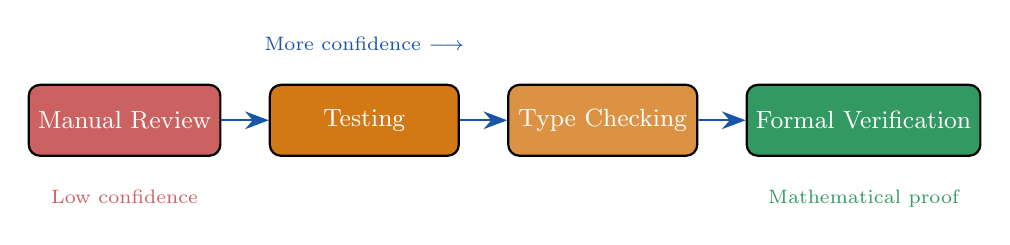
\begin{tikzpicture}[
  box/.style={draw, rounded corners, minimum width=2.4cm, minimum height=0.9cm,
              font=\small, text=white, thick},
  arr/.style={-{Stealth[length=3mm]}, thick, jugeoBlue}
]
  \node[box, fill=jugeoRed!70]                        (rev)  {Manual Review};
  \node[box, fill=jugeoOrange, right=0.6cm of rev]    (test) {Testing};
  \node[box, fill=jugeoOrange!80, right=0.6cm of test](type) {Type Checking};
  \node[box, fill=jugeoGreen!80, right=0.6cm of type] (fv)   {Formal Verification};

  \draw[arr] (rev)  -- (test);
  \draw[arr] (test) -- (type);
  \draw[arr] (type) -- (fv);

  \node[below=0.3cm of rev,  font=\scriptsize, text=jugeoRed!70]  {Low confidence};
  \node[below=0.3cm of fv,   font=\scriptsize, text=jugeoGreen!80]{Mathematical proof};
  \node[above=0.3cm of test, font=\scriptsize, text=jugeoBlue]    {More confidence $\longrightarrow$};
\end{tikzpicture}
\end{center}
\vfill
\begin{itemize}
  \item Each step catches \emph{more} bugs --- but demands \emph{more} effort
  \item Most Python projects stop at testing
  \item \jugmark{What would it take to go further?}
\end{itemize}
\end{frame}

%% Slide 5: What Is Formal Verification?
\begin{frame}
\frametitle{What Is Formal Verification?}
\begin{block}{Definition}
A \textbf{mathematical proof} that code meets its specification --- for \emph{all} possible inputs.
\end{block}
\vspace{0.4cm}
\begin{columns}[T]
\column{0.48\textwidth}
\begin{exampleblock}{What testing says}
  ``It didn't crash on \textbf{my} tests.''
\end{exampleblock}
\column{0.48\textwidth}
\begin{exampleblock}{What verification says}
  ``It \textbf{cannot} have this class of bug.''
\end{exampleblock}
\end{columns}
\vfill
\begin{itemize}
  \item Covers \emph{infinite} input space
  \item Eliminates entire bug categories by construction
  \item The gold standard --- but historically very expensive
\end{itemize}
\end{frame}

%% Slide 6: The Big Three — LEAN, Coq, F*
\begin{frame}
\frametitle{The Big Three --- LEAN, Coq, F*}
\begin{description}[\textbf{LEAN\,4}]
  \item[\textbf{LEAN\,4}] Interactive theorem prover from \textcolor{jugeoBlue}{Microsoft Research}.\\
    Dependent types, tactic-based proofs, growing math library.
  \item[\textbf{Coq}] Foundational proof assistant from \textcolor{jugeoBlue}{INRIA} (France).\\
    Calculus of Inductive Constructions, used in CompCert \& seL4.
  \item[\textbf{F*}] Effectful verification language from \textcolor{jugeoBlue}{MSR}.\\
    Refinement types + SMT (Z3), used in Project Everest (TLS).
\end{description}
\vfill
\begin{center}
  \small All three are \textbf{powerful}, \textbf{mature}, and \textbf{not Python}.
\end{center}
\end{frame}

%% Slide 7: How They Work — The Curry-Howard Idea
\begin{frame}
\frametitle{The Curry-Howard Idea}
\begin{center}
\Large ``Proofs are programs. Programs are proofs.''
\end{center}
\vspace{0.3cm}
\begin{columns}[T]
\column{0.45\textwidth}
\begin{block}{Logic side}
  \begin{itemize}
    \item Proposition $P$
    \item Proof of $P$
    \item $P \Rightarrow Q$
  \end{itemize}
\end{block}
\column{0.1\textwidth}
\begin{center}
\vspace{0.6cm}
\Large $\cong$
\end{center}
\column{0.45\textwidth}
\begin{block}{Programming side}
  \begin{itemize}
    \item Type \texttt{P}
    \item Value of type \texttt{P}
    \item Function \texttt{P -> Q}
  \end{itemize}
\end{block}
\end{columns}
\vfill
\begin{itemize}
  \item A proof of $P$ is a \textbf{program} that has type $P$
  \item If the program type-checks, the proof is \textbf{valid}
  \item Types \emph{enforce} correctness at compile time
\end{itemize}
\end{frame}

%% Slide 8: The Extraction Model
\begin{frame}
\frametitle{The Extraction Model}
\begin{center}
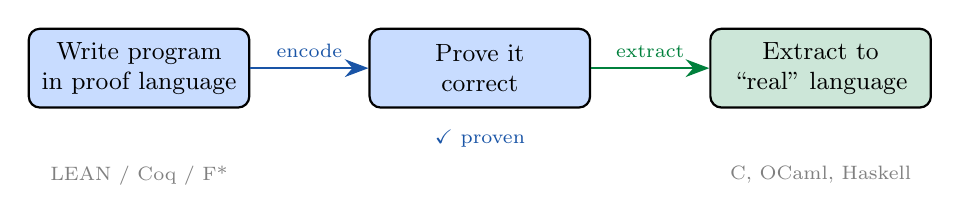
\begin{tikzpicture}[
  box/.style={draw, thick, rounded corners, minimum width=2.8cm, minimum height=1cm,
              font=\small, align=center},
  arr/.style={-{Stealth[length=3mm]}, thick}
]
  \node[box, fill=jugeoLight]                     (write) {Write program\\in proof language};
  \node[box, fill=jugeoLight, right=1.5cm of write]  (prove) {Prove it\\correct};
  \node[box, fill=jugeoGreen!20, right=1.5cm of prove]  (extract) {Extract to\\``real'' language};

  \draw[arr, jugeoBlue] (write)   -- node[above, font=\scriptsize]{encode} (prove);
  \draw[arr, jugeoGreen] (prove)  -- node[above, font=\scriptsize]{extract} (extract);

  \node[below=0.6cm of write,   font=\scriptsize, text=gray] {LEAN / Coq / F*};
  \node[below=0.6cm of extract, font=\scriptsize, text=gray] {C, OCaml, Haskell};

  \node[below=0.15cm of prove, font=\scriptsize, text=jugeoBlue] {$\checkmark$ proven};
\end{tikzpicture}
\end{center}
\vfill
\begin{itemize}
  \item You re-implement your algorithm inside the proof assistant
  \item Prove properties about that implementation
  \item Extract a certified executable --- in a language \emph{they} choose
  \item \jugmark{Your original code is never verified directly}
\end{itemize}
\end{frame}

%% Slide 9: Pain Point 1 — No Python
\begin{frame}
\frametitle{Pain Point 1 --- No Python}
\begin{center}
\begin{tabular}{l l}
  \toprule
  \textbf{Proof Assistant} & \textbf{Extraction Targets} \\
  \midrule
  LEAN 4  & C \\
  Coq     & OCaml, Haskell \\
  F*      & OCaml, F\#, C, Wasm \\
  \midrule
  \multicolumn{2}{c}{\textcolor{jugeoRed}{\textbf{Python?  Nowhere.}}} \\
  \bottomrule
\end{tabular}
\end{center}
\vfill
\begin{itemize}
  \item Python is the \textbf{\#1 language} (TIOBE, Stack Overflow, GitHub)
  \item ML, data science, web backends, scripting --- all Python
  \item Formal verification simply \textbf{ignores} the largest developer community
\end{itemize}
\end{frame}

%% Slide 10: Pain Point 2 — Rewrite Everything
\begin{frame}[fragile]
\frametitle{Pain Point 2 --- Rewrite Everything}
\begin{columns}[T]
\column{0.48\textwidth}
\begin{block}{Your Python}
\begin{lstlisting}
def merge_sort(xs):
    if len(xs) <= 1:
        return xs
    mid = len(xs) // 2
    left = merge_sort(xs[:mid])
    right = merge_sort(xs[mid:])
    return merge(left, right)
\end{lstlisting}
\end{block}
\column{0.48\textwidth}
\begin{block}{Rewritten in Coq}
\begin{lstlisting}[language=ML,
  morekeywords={Fixpoint,match,with,end,
    Defined,Program,let,in}]
Fixpoint merge_sort (xs: list nat)
  : list nat :=
  match xs with
  | [] => []
  | [x] => [x]
  | _ => let (l,r) :=
           split xs in
         merge (merge_sort l)
               (merge_sort r)
  end.
\end{lstlisting}
\end{block}
\end{columns}
\vfill
\begin{itemize}
  \item Two codebases to write, maintain, and keep in sync
  \item Your \emph{actual} Python is never verified
  \item \jugmark{Any divergence voids the guarantee}
\end{itemize}
\end{frame}

%% Slide 11: Pain Point 3 — Binary Trust
\begin{frame}
\frametitle{Pain Point 3 --- Binary Trust}
\begin{center}
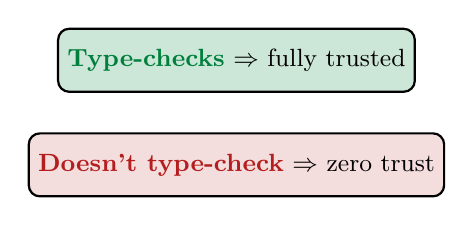
\begin{tikzpicture}[
  box/.style={draw, thick, rounded corners, minimum width=3cm, minimum height=0.8cm,
              font=\small, align=center}
]
  \node[box, fill=jugeoGreen!20]                        (pass) {\textcolor{jugeoGreen}{\textbf{Type-checks}} $\Rightarrow$ fully trusted};
  \node[box, fill=jugeoRed!15, below=0.5cm of pass] (fail) {\textcolor{jugeoRed}{\textbf{Doesn't type-check}} $\Rightarrow$ zero trust};
\end{tikzpicture}
\end{center}
\vspace{0.3cm}
\begin{itemize}
  \item There's no middle ground
  \item What about mixed evidence?
  \begin{itemize}
    \item ``Z3 proved the core math''
    \item ``Tests covered the edge cases''
    \item ``AI suggested the invariant''
    \item ``Manual review checked the IO''
  \end{itemize}
  \item \jugmark{No way to combine or account for these}
\end{itemize}
\end{frame}

%% Slide 12: Pain Point 4 — Opaque Failures
\begin{frame}
\frametitle{Pain Point 4 --- Opaque Failures}
\begin{columns}[T]
\column{0.48\textwidth}
\begin{alertblock}{F* says}
  \texttt{(error) Unknown assertion failed}\\[4pt]
  \footnotesize Z3 timed out. No explanation.\\
  No hint about \emph{what} went wrong.
\end{alertblock}
\column{0.48\textwidth}
\begin{alertblock}{Coq says}
  \texttt{Error: Tactic failure.}\\[4pt]
  \footnotesize Which sub-goal? Why?\\
  Good luck if you're not an expert.
\end{alertblock}
\end{columns}
\vfill
\begin{itemize}
  \item Failures are \textbf{unstructured} --- a string, not data
  \item No machine-readable explanation of \emph{what} failed
  \item No suggestion for \emph{how} to fix it
  \item \jugmark{Debugging proofs is harder than debugging code}
\end{itemize}
\end{frame}

%% Slide 13: Pain Point 5 — Python Effects Not Supported
\begin{frame}
\frametitle{Pain Point 5 --- Python Effects}
\begin{center}
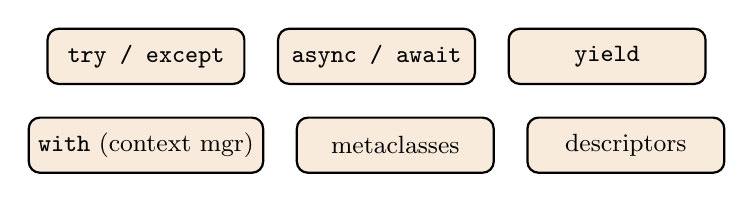
\begin{tikzpicture}[
  effect/.style={draw, thick, rounded corners, fill=jugeoOrange!15,
                 minimum width=2.5cm, minimum height=0.7cm, font=\small}
]
  \node[effect]                          (exc)  {\texttt{try / except}};
  \node[effect, right=0.4cm of exc]      (asy)  {\texttt{async / await}};
  \node[effect, right=0.4cm of asy]      (gen)  {\texttt{yield}};
  \node[effect, below=0.4cm of exc]      (ctx)  {\texttt{with} (context mgr)};
  \node[effect, right=0.4cm of ctx]      (meta) {metaclasses};
  \node[effect, right=0.4cm of meta]     (desc) {descriptors};
\end{tikzpicture}
\end{center}
\vfill
\begin{itemize}
  \item These are \emph{core} Python idioms, not exotic features
  \item LEAN, Coq, F* have no native model for any of them
  \item F* has \emph{some} effect support (monadic), but not Python's flavour
  \item \jugmark{You can't verify what you can't model}
\end{itemize}
\end{frame}

%% Slide 14: Pain Point 6 — AI Is External
\begin{frame}
\frametitle{Pain Point 6 --- AI Is External}
\begin{columns}[T]
\column{0.55\textwidth}
\begin{itemize}
  \item GitHub Copilot for LEAN exists
  \item LLM-based tactic suggestion is growing
  \item But AI is a \textbf{bolt-on}:
  \begin{itemize}
    \item No trust accounting
    \item AI proof step = formal proof step
    \item If the LLM hallucinates a lemma, \\the system accepts or rejects --- nothing in between
  \end{itemize}
\end{itemize}
\column{0.42\textwidth}
\begin{center}
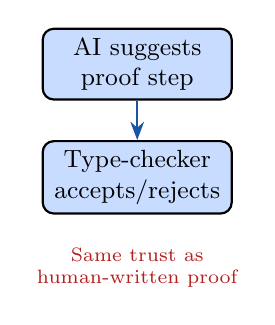
\begin{tikzpicture}[
  box/.style={draw, thick, rounded corners, minimum width=2.4cm,
              minimum height=0.8cm, font=\small, align=center}
]
  \node[box, fill=jugeoLight]                     (ai)  {AI suggests\\proof step};
  \node[box, fill=jugeoLight, below=0.5cm of ai]  (tc)  {Type-checker\\accepts/rejects};
  \node[below=0.3cm of tc, font=\scriptsize, text=jugeoRed, align=center]
    {Same trust as\\human-written proof};
  \draw[-{Stealth}, thick, jugeoBlue] (ai) -- (tc);
\end{tikzpicture}
\end{center}
\end{columns}
\vfill
\begin{itemize}
  \item \jugmark{No way to say ``AI contributed 40\%, Z3 proved 60\%''}
\end{itemize}
\end{frame}

%% Slide 15: Pain Point 7 — Module-Level Only
\begin{frame}
\frametitle{Pain Point 7 --- Module-Level Only}
\begin{center}
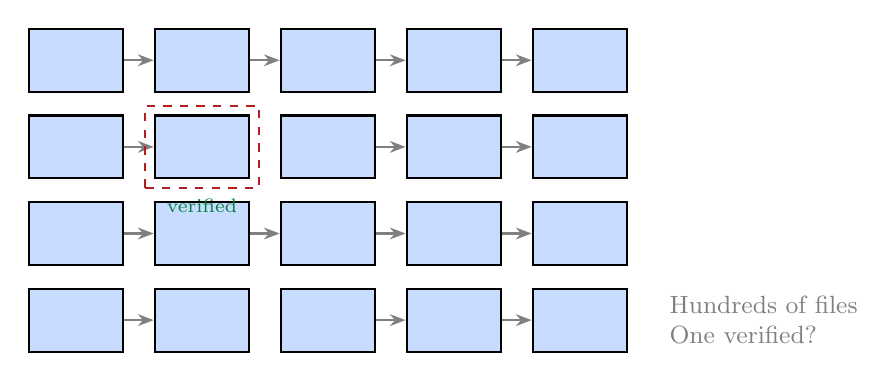
\begin{tikzpicture}[
  mod/.style={draw, thick, fill=jugeoLight, minimum width=1.2cm,
              minimum height=0.8cm, font=\scriptsize},
  arr/.style={-{Stealth[length=2mm]}, thick, gray}
]
  \foreach \i in {0,...,4} {
    \foreach \j in {0,...,3} {
      \node[mod] (m\i\j) at (1.6*\i, -1.1*\j) {};
    }
  }
  \draw[arr] (m00) -- (m10);  \draw[arr] (m10) -- (m20);
  \draw[arr] (m01) -- (m11);  \draw[arr] (m21) -- (m31);
  \draw[arr] (m02) -- (m12);  \draw[arr] (m12) -- (m22);
  \draw[arr] (m03) -- (m13);  \draw[arr] (m23) -- (m33);
  \draw[arr] (m30) -- (m40);  \draw[arr] (m31) -- (m41);
  \draw[arr] (m32) -- (m42);  \draw[arr] (m33) -- (m43);
  \draw[arr] (m20) -- (m30);
  \draw[arr] (m22) -- (m32);

  \node[draw=jugeoRed, thick, dashed, fit=(m11), inner sep=3pt, label={[font=\scriptsize,
    text=jugeoGreen]below:verified}] {};

  \node[right=0.4cm of m43, font=\small, text=gray, align=left]
    {Hundreds of files\\One verified?};
\end{tikzpicture}
\end{center}
\vfill
\begin{itemize}
  \item Proof assistants verify \emph{one module at a time}
  \item No built-in mechanism for cross-module reasoning
  \item Real projects have hundreds of interacting files
  \item \jugmark{Verification doesn't scale to whole projects}
\end{itemize}
\end{frame}

%% Slide 16: Pain Point 8 — Proofs Don't Ship With Code
\begin{frame}
\frametitle{Pain Point 8 --- Proofs Don't Ship}
\begin{center}
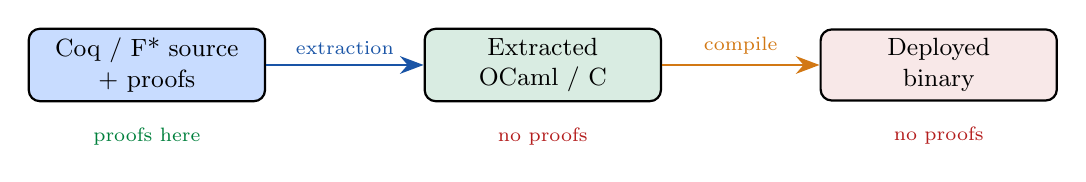
\begin{tikzpicture}[
  box/.style={draw, thick, rounded corners, minimum width=3cm, minimum height=0.9cm,
              font=\small, align=center},
  arr/.style={-{Stealth[length=3mm]}, thick}
]
  \node[box, fill=jugeoLight]                        (src)  {Coq / F* source\\+ proofs};
  \node[box, fill=jugeoGreen!15, right=2cm of src]   (ext)  {Extracted\\OCaml / C};
  \node[box, fill=jugeoRed!10, right=2cm of ext]     (dep)  {Deployed\\binary};

  \draw[arr, jugeoBlue]  (src) -- node[above, font=\scriptsize]{extraction} (ext);
  \draw[arr, jugeoOrange] (ext) -- node[above, font=\scriptsize]{compile} (dep);

  \node[below=0.2cm of src, font=\scriptsize, text=jugeoGreen] {proofs here};
  \node[below=0.2cm of ext, font=\scriptsize, text=jugeoRed]   {no proofs};
  \node[below=0.2cm of dep, font=\scriptsize, text=jugeoRed]   {no proofs};
\end{tikzpicture}
\end{center}
\vfill
\begin{itemize}
  \item Extracted code carries \textbf{no proof metadata}
  \item Deployed artifact has \textbf{no record} of how it was verified
  \item You must trust the build pipeline, not the artifact
  \item \jugmark{Proofs evaporate at extraction time}
\end{itemize}
\end{frame}

%% Slide 17: Summary of Pain Points
\begin{frame}
\frametitle{Summary --- 8 Pain Points}
\begin{center}
\small
\begin{tabular}{@{} r l l @{}}
  \toprule
  \textbf{\#} & \textbf{Pain Point} & \textbf{Impact} \\
  \midrule
  1 & No Python target              & Largest community excluded \\
  2 & Must rewrite everything       & Double codebase, drift risk \\
  3 & Binary trust (all or nothing) & Can't combine evidence sources \\
  4 & Opaque failures               & Unstructured, unhelpful errors \\
  5 & Python effects unsupported    & Core idioms can't be modeled \\
  6 & AI is a bolt-on               & No trust accounting for LLMs \\
  7 & Module-level only             & Doesn't scale to real projects \\
  8 & Proofs don't ship             & Artifact carries no evidence \\
  \bottomrule
\end{tabular}
\end{center}
\vfill
\begin{center}
\large These aren't minor inconveniences ---\\
they're \jugmark{structural limitations} of the extraction model.
\end{center}
\end{frame}

%% Slide 18: What If There Were a Better Way?
\begin{frame}
\frametitle{What If\ldots?}
\begin{center}
\vspace{0.5cm}
{\Large What if we could\ldots}\\[0.6cm]
\begin{itemize}
  \item[\textcolor{jugeoGreen}{$\checkmark$}] Verify \textbf{Python} directly --- no rewriting
  \item[\textcolor{jugeoGreen}{$\checkmark$}] Write proofs \textbf{in Python} --- no new language
  \item[\textcolor{jugeoGreen}{$\checkmark$}] Mix evidence sources with \textbf{trust accounting}
  \item[\textcolor{jugeoGreen}{$\checkmark$}] Ship proofs \textbf{with} the code --- not separate
  \item[\textcolor{jugeoGreen}{$\checkmark$}] Scale verification to \textbf{entire projects}
\end{itemize}
\vfill
{\large\itshape ``What if proofs traveled with the code?''}
\end{center}
\end{frame}

%% Slide 19: Enter JuGeo — Judgment Geometry
\begin{frame}
\frametitle{Enter JuGeo --- Judgment Geometry}
\begin{center}
\vspace{0.3cm}
{\LARGE \jugmark{JuGeo}}\\[0.5cm]
{\large A \textbf{proof-carrying Python} framework\\[4pt]
where proofs are \textcolor{jugeoGreen}{\textbf{geometric objects}}, not program terms.}
\end{center}
\vfill
\begin{columns}[T]
\column{0.48\textwidth}
\begin{block}{Traditional}
  Proof = a program that type-checks
\end{block}
\column{0.48\textwidth}
\begin{exampleblock}{JuGeo}
  Proof = a geometric object attached to code
\end{exampleblock}
\end{columns}
\vfill
\begin{center}
\small Proofs are \textbf{first-class data}, computed, composed, and shipped alongside your Python.
\end{center}
\end{frame}

%% Slide 20: Roadmap of This Talk
\begin{frame}
\frametitle{Roadmap}
\begin{center}
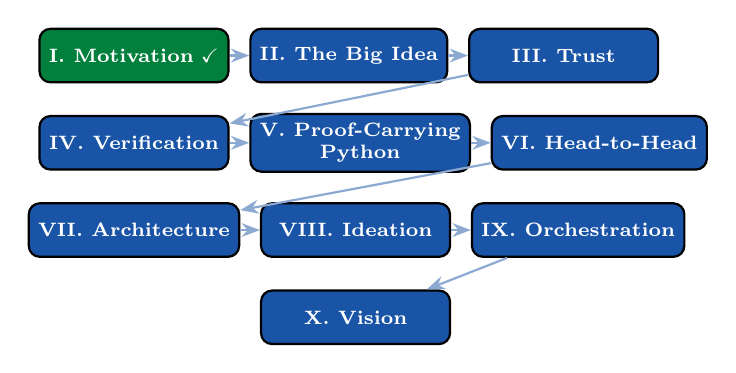
\begin{tikzpicture}[
  part/.style={draw, thick, rounded corners, minimum width=2.4cm, minimum height=0.68cm,
               font=\scriptsize\bfseries, align=center, text=white},
  done/.style={part, fill=jugeoGreen},
  todo/.style={part, fill=jugeoBlue}
]
  \node[done]                         (p1) {I.\ Motivation\;\checkmark};
  \node[todo, right=0.25cm of p1]     (p2) {II.\ The Big Idea};
  \node[todo, right=0.25cm of p2]     (p3) {III.\ Trust};

  \node[todo, below=0.4cm of p1]      (p4) {IV.\ Verification};
  \node[todo, right=0.25cm of p4]     (p5) {V.\ Proof-Carrying\\Python};
  \node[todo, right=0.25cm of p5]     (p6) {VI.\ Head-to-Head};

  \node[todo, below=0.4cm of p4]      (p7) {VII.\ Architecture};
  \node[todo, right=0.25cm of p7]     (p8) {VIII.\ Ideation};
  \node[todo, right=0.25cm of p8]     (p9) {IX.\ Orchestration};

  \node[todo, below=0.4cm of p8]      (p10) {X.\ Vision};

  \draw[-{Stealth}, thick, jugeoBlue!50] (p1) -- (p2);
  \draw[-{Stealth}, thick, jugeoBlue!50] (p2) -- (p3);
  \draw[-{Stealth}, thick, jugeoBlue!50] (p3) -- (p4);
  \draw[-{Stealth}, thick, jugeoBlue!50] (p4) -- (p5);
  \draw[-{Stealth}, thick, jugeoBlue!50] (p5) -- (p6);
  \draw[-{Stealth}, thick, jugeoBlue!50] (p6) -- (p7);
  \draw[-{Stealth}, thick, jugeoBlue!50] (p7) -- (p8);
  \draw[-{Stealth}, thick, jugeoBlue!50] (p8) -- (p9);
  \draw[-{Stealth}, thick, jugeoBlue!50] (p9) -- (p10);
\end{tikzpicture}
\end{center}
\vfill
\begin{center}
\small Part I complete --- next: \jugmark{The Big Idea} behind Judgment Geometry
\end{center}
\end{frame}

% Part II — The Big Idea: Geometry, Not Type Theory (Slides 21–40)
\providecommand{\jugmark}[1]{\textbf{\color{jugeoBlue}#1}}

% ---------------------------------------------------------------------------
% Slide 21: Section divider
% ---------------------------------------------------------------------------
\begin{frame}
\frametitle{}
\vfill
\begin{center}
  {\Huge\color{jugeoBlue}\textbf{Part II}}\\[12pt]
  {\LARGE\color{jugeoDark}The Big Idea: Geometry, Not Type Theory}\\[20pt]
  
\begin{tikzpicture}
    \draw[jugeoBlue, line width=2pt] (-3,0) -- (3,0);
  \end{tikzpicture}\\[12pt]
  {\large\color{gray}\itshape Replace proof terms with landscapes of evidence}
\end{center}
\vfill
\end{frame}

% ---------------------------------------------------------------------------
% Slide 22: Two Ways to Think About Proofs
% ---------------------------------------------------------------------------
\begin{frame}
\frametitle{Two Ways to Think About Proofs}
\begin{columns}[T]
\begin{column}{0.48\textwidth}
\begin{alertblock}{Traditional (Curry-Howard)}
  A proof is a \jugmark{PROGRAM}
  \begin{itemize}
    \item A term in a typed lambda calculus
    \item A syntax tree
    \item Grammar: right or wrong
  \end{itemize}
\end{alertblock}
\end{column}
\begin{column}{0.48\textwidth}
\begin{exampleblock}{JuGeo Approach}
  A proof is a \jugmark{MAP}
  \begin{itemize}
    \item A landscape of evidence
    \item Local measurements, globally consistent
    \item Geography: explore and chart
  \end{itemize}
\end{exampleblock}
\end{column}
\end{columns}
\vspace{10pt}
\begin{center}

\begin{tikzpicture}
  \node[fill=jugeoLight, rounded corners, inner sep=8pt, text width=10cm, align=center]
    {\itshape Think: checking grammar vs.\ charting a landscape};
\end{tikzpicture}
\end{center}
\end{frame}

% ---------------------------------------------------------------------------
% Slide 23: Analogy — Weather Forecasting
% ---------------------------------------------------------------------------
\begin{frame}
\frametitle{Analogy: Weather Forecasting}
\begin{center}
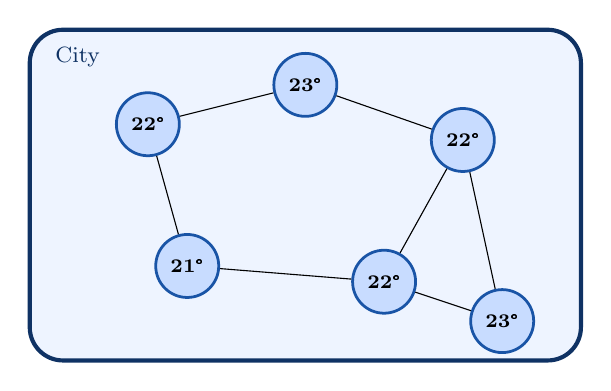
\begin{tikzpicture}[
    station/.style={circle, draw=jugeoBlue, fill=jugeoLight, minimum size=8mm,
                    font=\scriptsize\bfseries, line width=1pt},
    every edge/.style={draw=jugeoBlue!50, line width=0.8pt, dashed}
  ]
  % city outline
  \draw[jugeoDark, rounded corners=12pt, line width=1.5pt, fill=jugeoLight!30]
    (-3.5,-2) rectangle (3.5,2.2);
  \node[anchor=north west, font=\footnotesize\color{jugeoDark}] at (-3.3,2.1) {City};

  % stations
  \node[station] (s1) at (-2, 1)  {22\textdegree};
  \node[station] (s2) at ( 0, 1.5){23\textdegree};
  \node[station] (s3) at ( 2, 0.8){22\textdegree};
  \node[station] (s4) at (-1.5,-0.8){21\textdegree};
  \node[station] (s5) at ( 1,-1) {22\textdegree};
  \node[station] (s6) at ( 2.5,-1.5){23\textdegree};

  % edges
  \draw (s1)--(s2); \draw (s2)--(s3); \draw (s1)--(s4);
  \draw (s4)--(s5); \draw (s5)--(s3); \draw (s5)--(s6); \draw (s3)--(s6);
\end{tikzpicture}
\end{center}
\vspace{4pt}
\begin{itemize}
  \item Each station measures \jugmark{local} temperature
  \item Neighbors \jugmark{agree} $\Rightarrow$ glue into a global temperature map
  \item This idea is the heart of JuGeo's approach to proofs
\end{itemize}
\end{frame}

% ---------------------------------------------------------------------------
% Slide 24: Your Codebase Is a Map
% ---------------------------------------------------------------------------
\begin{frame}
\frametitle{Your Codebase Is a Map}
\begin{center}
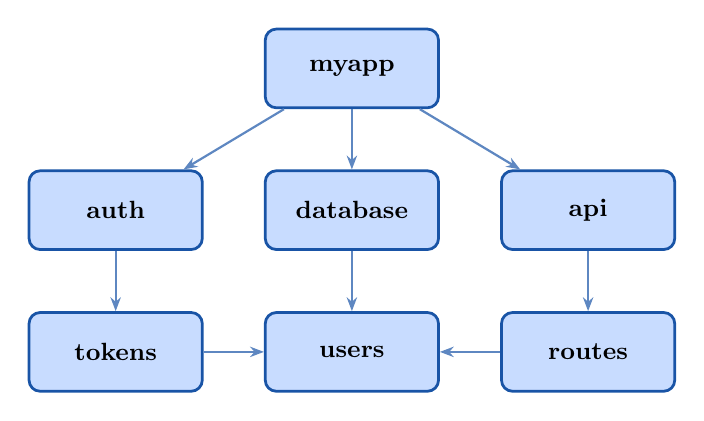
\begin{tikzpicture}[
    mod/.style={rectangle, rounded corners, draw=jugeoBlue, fill=jugeoLight,
                minimum width=22mm, minimum height=10mm, font=\small\bfseries,
                line width=1pt},
    conn/.style={-{Stealth[length=5pt]}, jugeoBlue!70, line width=0.8pt}
  ]
  \node[mod] (app)  at (0,2.4)  {myapp};
  \node[mod] (auth) at (-3,0.6) {auth};
  \node[mod] (db)   at (0,0.6)  {database};
  \node[mod] (api)  at (3,0.6)  {api};
  \node[mod] (tok)  at (-3,-1.2){tokens};
  \node[mod] (usr)  at (0,-1.2) {users};
  \node[mod] (rtr)  at (3,-1.2) {routes};

  \draw[conn] (app)--(auth);
  \draw[conn] (app)--(db);
  \draw[conn] (app)--(api);
  \draw[conn] (auth)--(tok);
  \draw[conn] (db)--(usr);
  \draw[conn] (api)--(rtr);
  \draw[conn] (rtr)--(usr);
  \draw[conn] (tok)--(usr);
\end{tikzpicture}
\end{center}
\vspace{6pt}
Each function, module, or class is a \jugmark{location} on the map.\\[4pt]
JuGeo calls these locations \jugmark{coordinates}.
\end{frame}

% ---------------------------------------------------------------------------
% Slide 25: What Is a Coordinate?
% ---------------------------------------------------------------------------
\begin{frame}
\frametitle{What Is a Coordinate?}
\begin{block}{Definition}
  A \jugmark{coordinate} is a specific place in your codebase:\\[2pt]
  \texttt{module\,.\,function\,.\,line}
\end{block}
\vspace{8pt}
\begin{exampleblock}{Example}
  \texttt{myapp.auth.validate\_token}\\[4pt]
  is a coordinate pointing to the \texttt{validate\_token} function\\
  inside the \texttt{auth} module of \texttt{myapp}.
\end{exampleblock}
\vspace{8pt}
\begin{center}
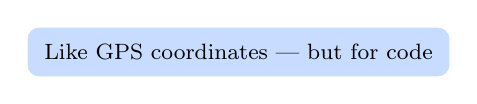
\begin{tikzpicture}
  \node[fill=jugeoLight, rounded corners, inner sep=6pt, font=\footnotesize]
    {Like GPS coordinates --- but for code};
\end{tikzpicture}
\end{center}
\end{frame}

% ---------------------------------------------------------------------------
% Slide 26: What Are Covers?
% ---------------------------------------------------------------------------
\begin{frame}
\frametitle{What Are Covers?}
\begin{columns}[T]
\begin{column}{0.55\textwidth}
\begin{block}{Definition}
  A \jugmark{cover} is a collection of test inputs that\\
  together cover the behavior space.
\end{block}
\vspace{6pt}
\begin{exampleblock}{Example}
  10 test inputs that exercise\\
  \textbf{all code paths} of a function.
\end{exampleblock}
\end{column}
\begin{column}{0.42\textwidth}
\begin{center}
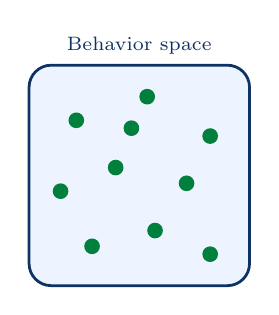
\begin{tikzpicture}[
    dot/.style={circle, fill=jugeoGreen, inner sep=2pt}
  ]
  \draw[jugeoDark, rounded corners=8pt, line width=1pt, fill=jugeoLight!30]
    (-1.4,-1.4) rectangle (1.4,1.4);
  \node[font=\scriptsize\color{jugeoDark}] at (0,1.65) {Behavior space};
  \foreach \x/\y in {-0.8/0.7, 0.1/1.0, 0.9/0.5, -1.0/-0.2, -0.3/0.1,
                      0.6/-0.1, -0.6/-0.9, 0.2/-0.7, 0.9/-1.0, -0.1/0.6} {
    \node[dot] at (\x,\y) {};
  }
\end{tikzpicture}\\[2pt]
{\scriptsize Enough stations $=$ full coverage}
\end{center}
\end{column}
\end{columns}
\end{frame}

% ---------------------------------------------------------------------------
% Slide 27: What Is Descent?
% ---------------------------------------------------------------------------
\begin{frame}
\frametitle{What Is Descent?}
\begin{center}
  \jugmark{Descent} $=$ gluing local truths into a global truth
\end{center}
\vspace{6pt}
\begin{center}
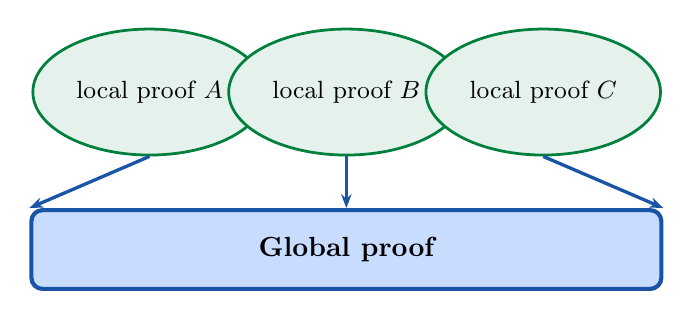
\begin{tikzpicture}[
    patch/.style={ellipse, draw=jugeoGreen, fill=jugeoGreen!10,
                  minimum width=28mm, minimum height=16mm,
                  line width=1pt, font=\small},
    arr/.style={-{Stealth[length=5pt]}, jugeoBlue, line width=1.2pt}
  ]
  \node[patch] (a) at (-2.5,0) {local proof $A$};
  \node[patch] (b) at ( 0,0)   {local proof $B$};
  \node[patch] (c) at ( 2.5,0) {local proof $C$};

  \node[rectangle, rounded corners, draw=jugeoBlue, fill=jugeoLight,
        minimum width=80mm, minimum height=10mm, line width=1.5pt,
        font=\bfseries] (g) at (0,-2) {Global proof};

  \draw[arr] (a.south) -- (g.north west);
  \draw[arr] (b.south) -- (g.north);
  \draw[arr] (c.south) -- (g.north east);
\end{tikzpicture}
\end{center}
\vspace{4pt}
\begin{itemize}
  \item Every test input confirms the spec \textcolor{jugeoGreen}{\checkmark}
  \item Test inputs cover everything \textcolor{jugeoGreen}{\checkmark}
  \item[$\Rightarrow$] Spec holds \jugmark{globally}
\end{itemize}
\end{frame}

% ---------------------------------------------------------------------------
% Slide 28: When Gluing Fails — Obstructions
% ---------------------------------------------------------------------------
\begin{frame}
\frametitle{When Gluing Fails --- Obstructions}
\begin{center}
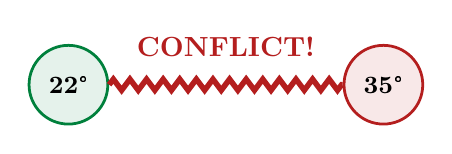
\begin{tikzpicture}[
    station/.style={circle, draw, minimum size=10mm, font=\small\bfseries, line width=1pt}
  ]
  \node[station, draw=jugeoGreen, fill=jugeoGreen!10] (a) at (-2,0) {22\textdegree};
  \node[station, draw=jugeoRed,   fill=jugeoRed!10]   (b) at ( 2,0) {35\textdegree};
  \draw[jugeoRed, line width=2pt, decorate,
        decoration={zigzag, segment length=6, amplitude=2}]
    (a) -- (b)
    node[midway, above=6pt, font=\bfseries\color{jugeoRed}] {CONFLICT!};
\end{tikzpicture}
\end{center}
\vspace{4pt}
\begin{alertblock}{Obstruction}
  Neighboring proofs \textbf{contradict} each other at overlaps.
\end{alertblock}
\vspace{4pt}
\begin{itemize}
  \item Traditional tools: ``Unknown'' or ``timeout'' --- no explanation
  \item JuGeo: a structured \jugmark{mathematical object}\\
        that tells you \textbf{what} broke and \textbf{how} to fix it
\end{itemize}
\end{frame}

% ---------------------------------------------------------------------------
% Slide 29: The Core Insight
% ---------------------------------------------------------------------------
\begin{frame}
\frametitle{The Core Insight}
\begin{columns}[T]
\begin{column}{0.48\textwidth}
\begin{alertblock}{Traditional}
  \centering
  Proof $=$ one big term\\[6pt]
  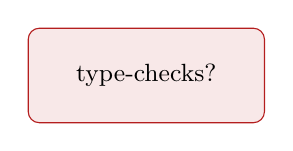
\begin{tikzpicture}
    \node[rectangle, draw=jugeoRed, fill=jugeoRed!10, rounded corners,
          minimum width=30mm, minimum height=12mm, font=\small]
      {type-checks?};
  \end{tikzpicture}\\[6pt]
  \textbf{Yes} or \textbf{No}
\end{alertblock}
\end{column}
\begin{column}{0.48\textwidth}
\begin{exampleblock}{JuGeo}
  \centering
  Proof $=$ local evidence\\[6pt]
  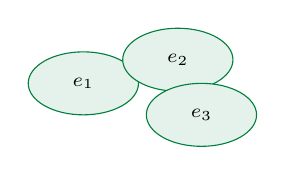
\begin{tikzpicture}
    \node[ellipse, draw=jugeoGreen, fill=jugeoGreen!10,
          minimum width=14mm, minimum height=8mm, font=\scriptsize] (e1) at (-0.9,0) {$e_1$};
    \node[ellipse, draw=jugeoGreen, fill=jugeoGreen!10,
          minimum width=14mm, minimum height=8mm, font=\scriptsize] (e2) at (0.3,0.3) {$e_2$};
    \node[ellipse, draw=jugeoGreen, fill=jugeoGreen!10,
          minimum width=14mm, minimum height=8mm, font=\scriptsize] (e3) at (0.6,-0.4) {$e_3$};
  \end{tikzpicture}\\[6pt]
  Glued by \jugmark{descent}
\end{exampleblock}
\end{column}
\end{columns}
\vspace{10pt}
\begin{center}
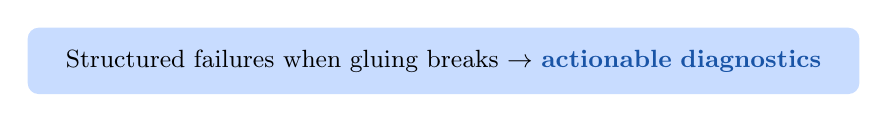
\begin{tikzpicture}
  \node[fill=jugeoLight, rounded corners, inner sep=8pt, text width=10cm, align=center,
        font=\small]
    {Structured failures when gluing breaks $\rightarrow$
     \jugmark{actionable diagnostics}};
\end{tikzpicture}
\end{center}
\end{frame}

% ---------------------------------------------------------------------------
% Slide 30: The Judgment — JuGeo's Central Object
% ---------------------------------------------------------------------------
\begin{frame}
\frametitle{The Judgment --- JuGeo's Central Object}
\begin{center}
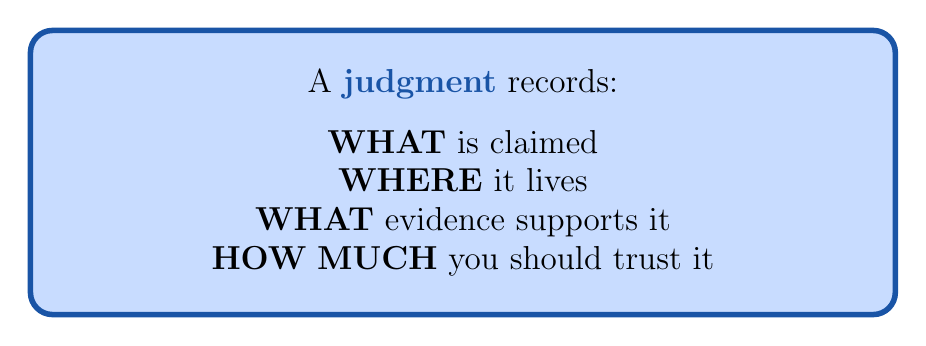
\begin{tikzpicture}
  \node[rectangle, rounded corners=8pt, draw=jugeoBlue, fill=jugeoLight,
        line width=2pt, inner sep=14pt, font=\large, text width=10cm, align=center]
    {A \jugmark{judgment} records:\\[8pt]
     \textbf{WHAT} is claimed\\
     \textbf{WHERE} it lives\\
     \textbf{WHAT} evidence supports it\\
     \textbf{HOW MUCH} you should trust it};
\end{tikzpicture}
\end{center}
\vspace{10pt}
\begin{itemize}
  \item Not a boolean (\texttt{True}/\texttt{False})
  \item Not a proof term (a lambda expression)
  \item An \jugmark{8-component record} --- the central data structure of JuGeo
\end{itemize}
\end{frame}

% ---------------------------------------------------------------------------
% Slide 31: The Judgment 8-Tuple — Overview
% ---------------------------------------------------------------------------
\begin{frame}
\frametitle{The Judgment 8-Tuple}
\begin{center}
  {\Large $\mathcal{J} = (c,\;\varphi,\;A,\;E,\;O,\;B,\;T,\;\Pi)$}
\end{center}
\vspace{6pt}
\begin{center}
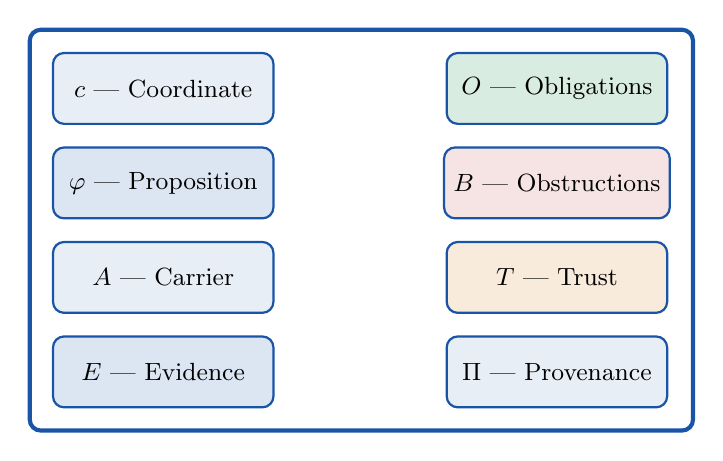
\begin{tikzpicture}[
    comp/.style={rectangle, rounded corners, minimum width=28mm, minimum height=9mm,
                 draw=jugeoBlue, line width=0.8pt, font=\small, align=center}
  ]
  \node[comp, fill=jugeoBlue!10]   (c)  at (-4, 1.2) {$c$ --- Coordinate};
  \node[comp, fill=jugeoBlue!15]   (ph) at (-4, 0)   {$\varphi$ --- Proposition};
  \node[comp, fill=jugeoBlue!10]   (a)  at (-4,-1.2) {$A$ --- Carrier};
  \node[comp, fill=jugeoBlue!15]   (e)  at (-4,-2.4) {$E$ --- Evidence};
  \node[comp, fill=jugeoGreen!15]  (o)  at ( 1, 1.2) {$O$ --- Obligations};
  \node[comp, fill=jugeoRed!12]    (b)  at ( 1, 0)   {$B$ --- Obstructions};
  \node[comp, fill=jugeoOrange!15] (t)  at ( 1,-1.2) {$T$ --- Trust};
  \node[comp, fill=jugeoBlue!10]   (pi) at ( 1,-2.4) {$\Pi$ --- Provenance};

  \node[draw=jugeoBlue, rounded corners, line width=1.5pt,
        fit=(c)(ph)(a)(e)(o)(b)(t)(pi), inner sep=8pt] {};
\end{tikzpicture}
\end{center}
\vspace{4pt}
\begin{center}
  {\footnotesize We'll walk through each component next.}
\end{center}
\end{frame}

% ---------------------------------------------------------------------------
% Slide 32: Component 1 — Coordinate (c)
% ---------------------------------------------------------------------------
\begin{frame}
\frametitle{Component 1: Coordinate ($c$)}
\begin{block}{\jugmark{WHERE} in the codebase}
  A coordinate pinpoints the exact location being verified.
\end{block}
\vspace{6pt}
\begin{exampleblock}{Example}
  \texttt{myapp.auth.validate\_token.line\_42}
\end{exampleblock}
\vspace{6pt}
\begin{center}
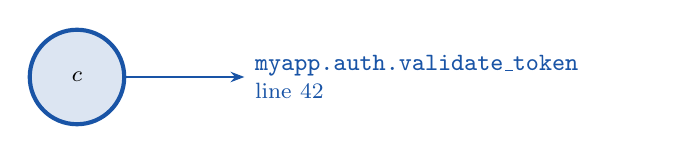
\begin{tikzpicture}
  \node[circle, draw=jugeoBlue, fill=jugeoBlue!15, minimum size=12mm,
        font=\footnotesize\bfseries, line width=1.5pt] (pin) {$c$};
  \draw[-{Stealth[length=5pt]}, jugeoBlue, line width=1pt]
    (pin.east) -- ++(1.5,0)
    node[right, font=\small, text width=5cm]
      {\texttt{myapp.auth.validate\_token}\\[-1pt]\footnotesize line 42};
\end{tikzpicture}
\end{center}
\vspace{6pt}
\begin{center}
  {\small Like \jugmark{GPS coordinates} --- but for code.}
\end{center}
\end{frame}

% ---------------------------------------------------------------------------
% Slide 33: Component 2 — Proposition (φ)
% ---------------------------------------------------------------------------
\begin{frame}
\frametitle{Component 2: Proposition ($\varphi$)}
\begin{block}{\jugmark{WHAT} is claimed}
  The logical statement being verified at coordinate $c$.
\end{block}
\vspace{8pt}
\begin{exampleblock}{Example}
  \begin{center}
    ``\texttt{validate\_token} returns a non-negative integer''\\[6pt]
    $\varphi \;\equiv\; \forall\, x.\;\texttt{validate\_token}(x) \geq 0$
  \end{center}
\end{exampleblock}
\vspace{8pt}
\begin{center}
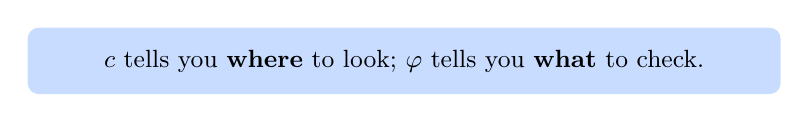
\begin{tikzpicture}
  \node[fill=jugeoLight, rounded corners, inner sep=8pt, font=\small, text width=9cm,
        align=center]
    {$c$ tells you \textbf{where} to look; $\varphi$ tells you \textbf{what} to check.};
\end{tikzpicture}
\end{center}
\end{frame}

% ---------------------------------------------------------------------------
% Slide 34: Component 3 — Carrier (A)
% ---------------------------------------------------------------------------
\begin{frame}
\frametitle{Component 3: Carrier ($A$)}
\begin{block}{\jugmark{TYPE} of the claim}
  The mathematical domain in which $\varphi$ is stated.
\end{block}
\vspace{6pt}
\begin{exampleblock}{Example}
  \begin{center}
    $A = \texttt{int} \to \texttt{int}$\\[6pt]
    The function maps integers to integers.
  \end{center}
\end{exampleblock}
\vspace{8pt}
\begin{itemize}
  \item JuGeo's version of \emph{dependent types}
  \item Determines which proof methods are valid
  \item Enables the system to compose proofs across modules
\end{itemize}
\end{frame}

% ---------------------------------------------------------------------------
% Slide 35: Component 4 — Evidence Bundle (E)
% ---------------------------------------------------------------------------
\begin{frame}
\frametitle{Component 4: Evidence Bundle ($E$)}
\begin{block}{\jugmark{THE PROOF} --- from multiple channels}
  Not one proof, but a \textbf{bundle} of evidence.
\end{block}
\vspace{4pt}
\begin{center}
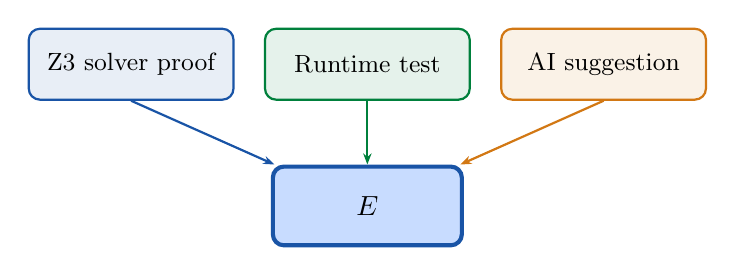
\begin{tikzpicture}[
    ev/.style={rectangle, rounded corners, draw, minimum width=26mm,
               minimum height=9mm, font=\small, line width=0.8pt}
  ]
  \node[ev, draw=jugeoBlue, fill=jugeoBlue!10]   (z3)  at (-3,0) {Z3 solver proof};
  \node[ev, draw=jugeoGreen, fill=jugeoGreen!10]  (rt)  at (0,0)  {Runtime test};
  \node[ev, draw=jugeoOrange, fill=jugeoOrange!10] (ai) at (3,0)  {AI suggestion};

  \node[rectangle, rounded corners, draw=jugeoBlue, fill=jugeoLight,
        minimum width=24mm, minimum height=10mm, font=\bfseries,
        line width=1.5pt] (e) at (0,-1.8) {$E$};

  \draw[-{Stealth[length=4pt]}, jugeoBlue, line width=0.8pt] (z3.south) -- (e);
  \draw[-{Stealth[length=4pt]}, jugeoGreen, line width=0.8pt] (rt.south) -- (e);
  \draw[-{Stealth[length=4pt]}, jugeoOrange, line width=0.8pt] (ai.south) -- (e);
\end{tikzpicture}
\end{center}
\vspace{4pt}
\begin{center}
  {\small Like having \jugmark{multiple witnesses} in court---\\[2pt]
   each adds confidence from a different angle.}
\end{center}
\end{frame}

% ---------------------------------------------------------------------------
% Slide 36: Component 5 — Obligations (O)
% ---------------------------------------------------------------------------
\begin{frame}
\frametitle{Component 5: Obligations ($O$)}
\begin{block}{\jugmark{TODO list} --- what still needs proving}
  Obligations are proof goals that remain open.
\end{block}
\vspace{6pt}
\begin{center}
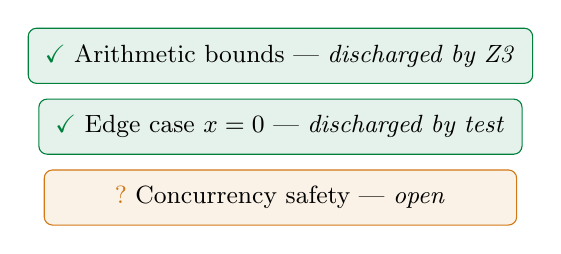
\begin{tikzpicture}[
    ob/.style={rectangle, rounded corners=3pt, font=\small, minimum width=60mm,
               minimum height=7mm, align=left, inner xsep=6pt}
  ]
  \node[ob, draw=jugeoGreen, fill=jugeoGreen!10]
    (o1) at (0, 0.9) {\textcolor{jugeoGreen}{\checkmark}~Arithmetic bounds --- \emph{discharged by Z3}};
  \node[ob, draw=jugeoGreen, fill=jugeoGreen!10]
    (o2) at (0, 0)   {\textcolor{jugeoGreen}{\checkmark}~Edge case $x=0$ --- \emph{discharged by test}};
  \node[ob, draw=jugeoOrange, fill=jugeoOrange!10]
    (o3) at (0,-0.9) {\textcolor{jugeoOrange}{?}~Concurrency safety --- \emph{open}};
\end{tikzpicture}
\end{center}
\vspace{6pt}
\begin{itemize}
  \item Some discharged by \jugmark{Z3}, some by \jugmark{tests}
  \item Open obligations are tracked, not forgotten
  \item JuGeo never silently drops proof goals
\end{itemize}
\end{frame}

% ---------------------------------------------------------------------------
% Slide 37: Component 6 — Obstructions (B)
% ---------------------------------------------------------------------------
\begin{frame}
\frametitle{Component 6: Obstructions ($B$)}
\begin{block}{Persistent \jugmark{blockers}}
  When something \textbf{can't} be proved, the failure itself becomes data.
\end{block}
\vspace{4pt}
\begin{columns}[T]
\begin{column}{0.48\textwidth}
\begin{alertblock}{F* / Lean}
  \centering
  \texttt{Unknown}\\[4pt]
  \texttt{(timeout after 30s)}\\[8pt]
  {\footnotesize No explanation.}
\end{alertblock}
\end{column}
\begin{column}{0.48\textwidth}
\begin{exampleblock}{JuGeo}
  \centering
  \texttt{Obstruction:}\\[2pt]
  {\footnotesize overlap at \texttt{auth$\cap$db}}\\
  {\footnotesize type mismatch \texttt{int/str}}\\[4pt]
  {\footnotesize \jugmark{What} broke $+$ \jugmark{how} to fix it.}
\end{exampleblock}
\end{column}
\end{columns}
\vspace{6pt}
\begin{center}
  {\small Obstructions are \jugmark{first-class mathematical objects},\\
   not error messages.}
\end{center}
\end{frame}

% ---------------------------------------------------------------------------
% Slide 38: Component 7 — Trust (T)
% ---------------------------------------------------------------------------
\begin{frame}
\frametitle{Component 7: Trust ($T$)}
\begin{block}{\jugmark{HOW MUCH} to trust this judgment}
  Not binary! A 7-level algebra.
\end{block}
\vspace{4pt}
\begin{center}
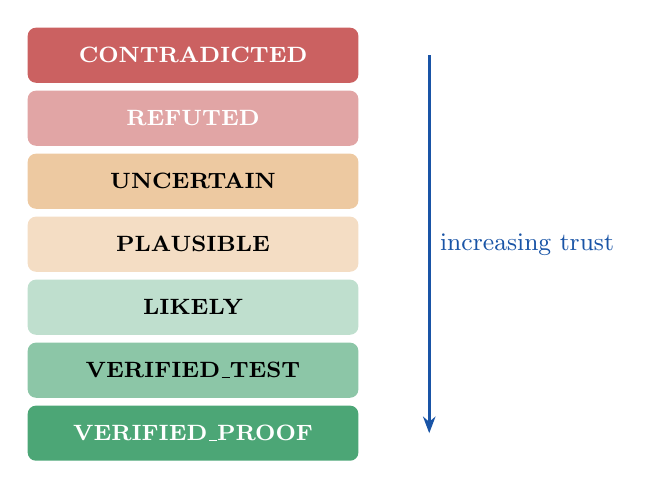
\begin{tikzpicture}[
    lev/.style={rectangle, rounded corners=3pt, minimum width=42mm,
                minimum height=7mm, font=\footnotesize\bfseries, align=center,
                line width=0.6pt}
  ]
  \node[lev, fill=jugeoRed!70, text=white]    at (0, 2.4) {CONTRADICTED};
  \node[lev, fill=jugeoRed!40, text=white]    at (0, 1.6) {REFUTED};
  \node[lev, fill=jugeoOrange!40]              at (0, 0.8) {UNCERTAIN};
  \node[lev, fill=jugeoOrange!25]              at (0, 0)   {PLAUSIBLE};
  \node[lev, fill=jugeoGreen!25]               at (0,-0.8) {LIKELY};
  \node[lev, fill=jugeoGreen!45]               at (0,-1.6) {VERIFIED\_TEST};
  \node[lev, fill=jugeoGreen!70, text=white]   at (0,-2.4) {VERIFIED\_PROOF};

  \draw[-{Stealth[length=6pt]}, line width=1.2pt, jugeoBlue]
    (3, 2.4) -- (3,-2.4) node[midway, right, font=\small] {increasing trust};
\end{tikzpicture}
\end{center}
\vspace{4pt}
\begin{center}
  {\footnotesize Deep dive in \textbf{Part III}.}
\end{center}
\end{frame}

% ---------------------------------------------------------------------------
% Slide 39: Component 8 — Provenance (Π)
% ---------------------------------------------------------------------------
\begin{frame}
\frametitle{Component 8: Provenance ($\Pi$)}
\begin{block}{\jugmark{WHO} produced this judgment and \jugmark{HOW}}
  Full audit trail for every piece of evidence.
\end{block}
\vspace{6pt}
\begin{center}
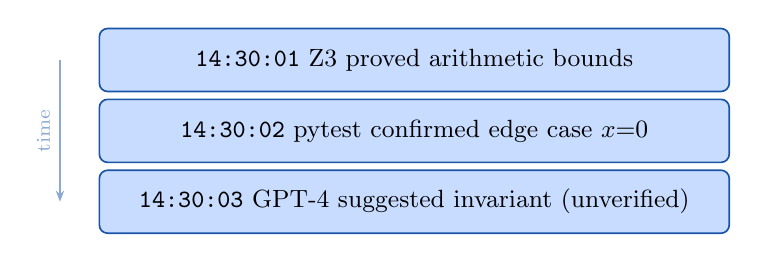
\begin{tikzpicture}[
    entry/.style={rectangle, rounded corners=3pt, draw=jugeoBlue,
                  fill=jugeoLight, minimum width=80mm, minimum height=8mm,
                  font=\small, align=left, inner xsep=6pt, line width=0.6pt}
  ]
  \node[entry] (p1) at (0, 0.9)
    {\texttt{14:30:01}~Z3 proved arithmetic bounds};
  \node[entry] (p2) at (0, 0)
    {\texttt{14:30:02}~pytest confirmed edge case $x{=}0$};
  \node[entry] (p3) at (0,-0.9)
    {\texttt{14:30:03}~GPT-4 suggested invariant (unverified)};

  \draw[-{Stealth[length=4pt]}, jugeoBlue!50, line width=0.6pt]
    (-4.5,0.9)--(-4.5,-0.9) node[midway, left, font=\scriptsize, rotate=90, anchor=south]
    {time};
\end{tikzpicture}
\end{center}
\vspace{6pt}
\begin{itemize}
  \item Every evidence channel is \jugmark{timestamped} and \jugmark{attributed}
  \item Enables reproducibility and blame tracking
\end{itemize}
\end{frame}

% ---------------------------------------------------------------------------
% Slide 40: Putting It All Together
% ---------------------------------------------------------------------------
\begin{frame}
\frametitle{Putting It All Together}
\begin{center}
  {\small A judgment for \texttt{validate\_token}:}
\end{center}
\vspace{2pt}
\begin{center}
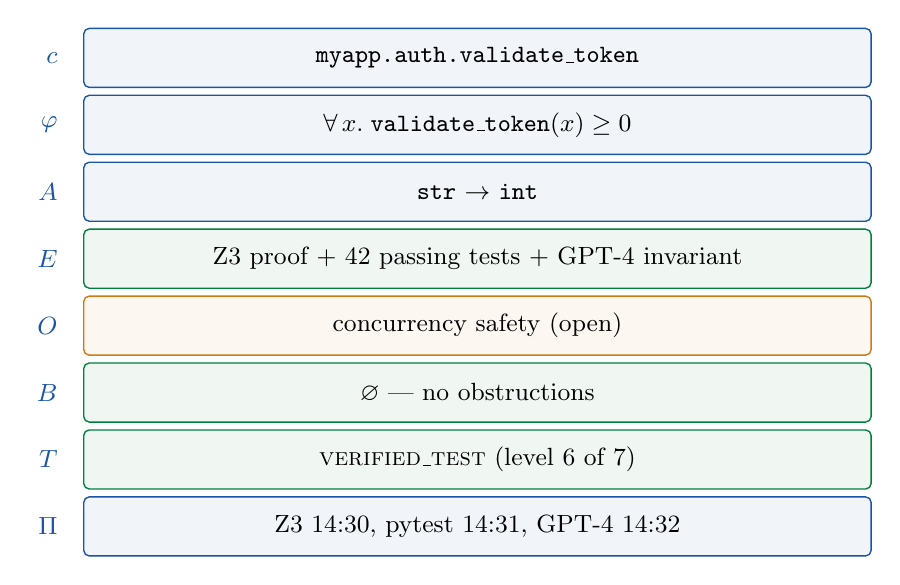
\begin{tikzpicture}[
    row/.style={rectangle, rounded corners=2pt, minimum width=100mm,
                minimum height=7.5mm, font=\small, align=left, inner xsep=6pt,
                line width=0.5pt, anchor=west},
    lab/.style={font=\small\bfseries\color{jugeoBlue}, anchor=east}
  ]
  \def\yy{0.85}
  \node[lab] at (-0.2, 3*\yy) {$c$};
  \node[row, draw=jugeoBlue, fill=jugeoBlue!6]  at (0, 3*\yy)
    {\texttt{myapp.auth.validate\_token}};

  \node[lab] at (-0.2, 2*\yy) {$\varphi$};
  \node[row, draw=jugeoBlue, fill=jugeoBlue!6]  at (0, 2*\yy)
    {$\forall\, x.\;\texttt{validate\_token}(x) \geq 0$};

  \node[lab] at (-0.2, 1*\yy) {$A$};
  \node[row, draw=jugeoBlue, fill=jugeoBlue!6]  at (0, 1*\yy)
    {\texttt{str} $\to$ \texttt{int}};

  \node[lab] at (-0.2, 0*\yy) {$E$};
  \node[row, draw=jugeoGreen, fill=jugeoGreen!6] at (0, 0*\yy)
    {Z3 proof $+$ 42 passing tests $+$ GPT-4 invariant};

  \node[lab] at (-0.2,-1*\yy) {$O$};
  \node[row, draw=jugeoOrange, fill=jugeoOrange!6] at (0,-1*\yy)
    {concurrency safety (open)};

  \node[lab] at (-0.2,-2*\yy) {$B$};
  \node[row, draw=jugeoGreen, fill=jugeoGreen!6] at (0,-2*\yy)
    {$\varnothing$ --- no obstructions};

  \node[lab] at (-0.2,-3*\yy) {$T$};
  \node[row, draw=jugeoGreen, fill=jugeoGreen!6] at (0,-3*\yy)
    {\textsc{verified\_test} (level 6 of 7)};

  \node[lab] at (-0.2,-4*\yy) {$\Pi$};
  \node[row, draw=jugeoBlue, fill=jugeoBlue!6]  at (0,-4*\yy)
    {Z3 14:30, pytest 14:31, GPT-4 14:32};
\end{tikzpicture}
\end{center}
\vspace{2pt}
\begin{center}
  {\small This is what \jugmark{JuGeo produces} for every verified location.}
\end{center}
\end{frame}

% Part III — The Trust Algebra (Slides 41–60)
\providecommand{\jugmark}[1]{\textbf{\color{jugeoBlue}#1}}

% ---------------------------------------------------------------------------
% Slide 41: Section divider
% ---------------------------------------------------------------------------
\begin{frame}
\frametitle{}
\vfill
\begin{center}
  {\Huge\color{jugeoBlue}\textbf{Part III}}\\[12pt]
  {\LARGE\color{jugeoDark}Trust --- The Key Innovation}\\[20pt]
  
\begin{tikzpicture}
    \draw[jugeoBlue, line width=2pt] (-3,0) -- (3,0);
  \end{tikzpicture}\\[12pt]
  {\large\color{gray}\itshape Not all evidence is created equal}
\end{center}
\vfill
\end{frame}

% ---------------------------------------------------------------------------
% Slide 42: The Problem with Binary Trust
% ---------------------------------------------------------------------------
\begin{frame}
\frametitle{The Problem with Binary Trust}
\begin{center}
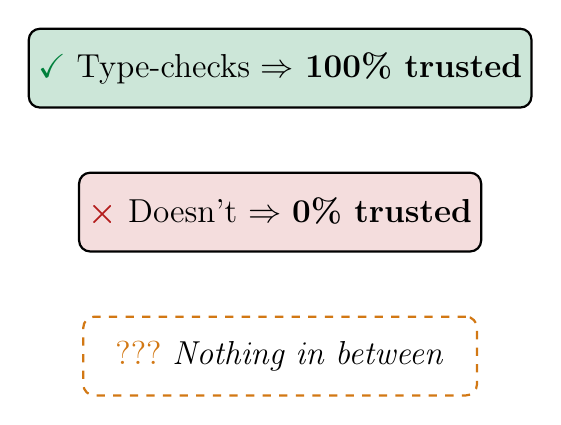
\begin{tikzpicture}[
  box/.style={draw, thick, rounded corners, minimum width=5cm,
              minimum height=1cm, font=\large, align=center}
]
  \node[box, fill=jugeoGreen!20] (yes) {\textcolor{jugeoGreen}{\textbf{\checkmark}}~Type-checks $\Rightarrow$ \textbf{100\% trusted}};
  \node[box, fill=jugeoRed!15, below=0.8cm of yes]
        (no)  {\textcolor{jugeoRed}{\textbf{\texttimes}}~Doesn't $\Rightarrow$ \textbf{0\% trusted}};
  \node[draw=jugeoOrange, dashed, thick, rounded corners,
        minimum width=5cm, minimum height=1cm,
        below=0.8cm of no, font=\large, align=center]
        (mid) {\textcolor{jugeoOrange}{???}~\emph{Nothing in between}};
\end{tikzpicture}
\end{center}
\vfill
\begin{itemize}
  \item LEAN / Coq / F*: proof accepted or rejected --- that's it
  \item Real-world evidence has \jugmark{degrees of confidence}
  \item Z3 proved 80\%, tests covered 15\%, expert reviewed 5\% --- where does that go?
\end{itemize}
\end{frame}

% ---------------------------------------------------------------------------
% Slide 43: Analogy — Courtroom Evidence
% ---------------------------------------------------------------------------
\begin{frame}
\frametitle{Analogy --- Courtroom Evidence}
\begin{center}
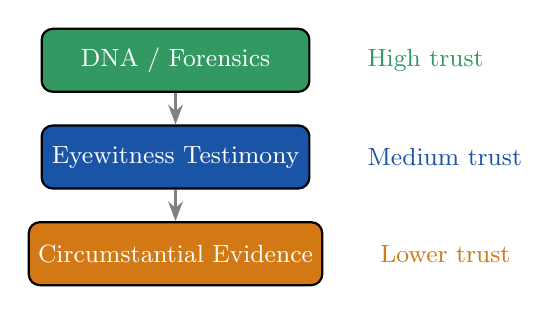
\begin{tikzpicture}[
  ev/.style={draw, thick, rounded corners, minimum width=3.4cm,
             minimum height=0.8cm, font=\small, align=center, text=white},
  arr/.style={-{Stealth[length=2.5mm]}, thick, gray}
]
  \node[ev, fill=jugeoGreen!80]                     (dna)  {DNA / Forensics};
  \node[ev, fill=jugeoBlue,  below=0.4cm of dna]    (eye)  {Eyewitness Testimony};
  \node[ev, fill=jugeoOrange, below=0.4cm of eye]   (circ) {Circumstantial Evidence};

  \node[right=0.6cm of dna,  font=\small, text=jugeoGreen!80]  {High trust};
  \node[right=0.6cm of eye,  font=\small, text=jugeoBlue]      {Medium trust};
  \node[right=0.6cm of circ, font=\small, text=jugeoOrange]    {Lower trust};

  \draw[arr] (dna)  -- (eye);
  \draw[arr] (eye)  -- (circ);
\end{tikzpicture}
\end{center}
\vfill
\begin{itemize}
  \item A jury doesn't rely on a single witness
  \item They \textbf{weigh} multiple channels of evidence
  \item The verdict reflects the \emph{combined} picture
  \item \jugmark{JuGeo works the same way for code verification}
\end{itemize}
\end{frame}

% ---------------------------------------------------------------------------
% Slide 44: JuGeo's Evidence Channels
% ---------------------------------------------------------------------------
\begin{frame}
\frametitle{JuGeo's Evidence Channels}
\begin{center}
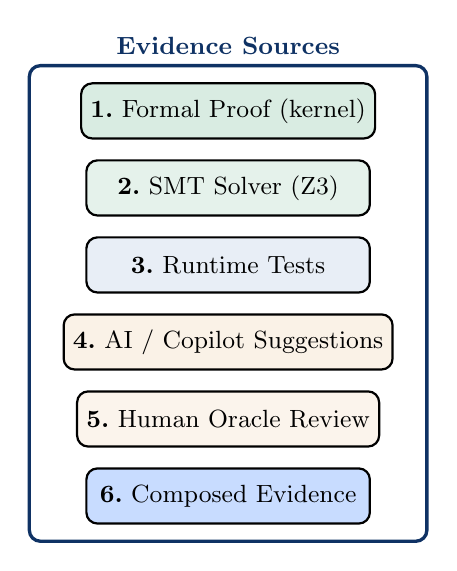
\begin{tikzpicture}[
  ch/.style={draw, thick, rounded corners, minimum width=3.6cm,
             minimum height=0.7cm, font=\small, align=center},
  arr/.style={-{Stealth[length=2mm]}, thick, jugeoBlue!50}
]
  \node[ch, fill=jugeoGreen!15]                       (k) {\textbf{1.}~Formal Proof (kernel)};
  \node[ch, fill=jugeoGreen!10, below=0.25cm of k]   (z) {\textbf{2.}~SMT Solver (Z3)};
  \node[ch, fill=jugeoBlue!10,  below=0.25cm of z]   (t) {\textbf{3.}~Runtime Tests};
  \node[ch, fill=jugeoOrange!10,below=0.25cm of t]   (a) {\textbf{4.}~AI / Copilot Suggestions};
  \node[ch, fill=jugeoOrange!8, below=0.25cm of a]   (h) {\textbf{5.}~Human Oracle Review};
  \node[ch, fill=jugeoLight,    below=0.25cm of h]   (c) {\textbf{6.}~Composed Evidence};

  \node[draw=jugeoDark, very thick, rounded corners,
        fit=(k)(z)(t)(a)(h)(c), inner xsep=12pt, inner ysep=6pt,
        label={[font=\small\bfseries, text=jugeoDark]above:Evidence Sources}] {};
\end{tikzpicture}
\end{center}
\vfill
\begin{itemize}
  \item Each channel produces evidence with a \textbf{different trust level}
  \item JuGeo tracks \emph{which} channel justified \emph{which} claim
  \item \jugmark{No channel is ignored; no channel is unconditionally trusted}
\end{itemize}
\end{frame}

% ---------------------------------------------------------------------------
% Slide 45: The Seven Trust Levels
% ---------------------------------------------------------------------------
\begin{frame}
\frametitle{The Seven Trust Levels}
\begin{center}
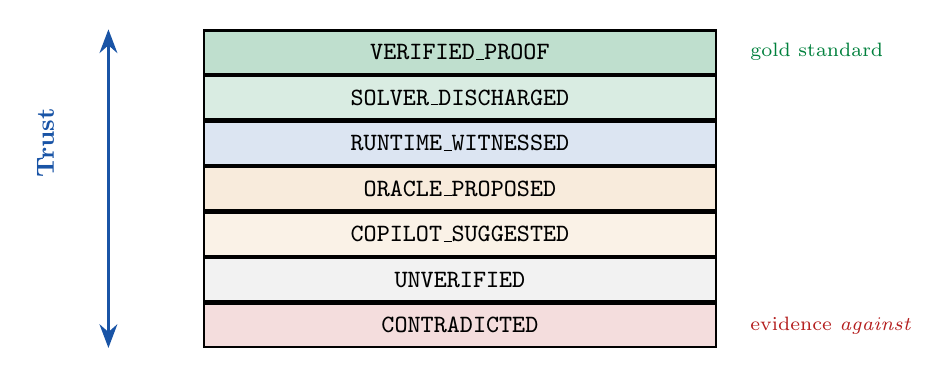
\begin{tikzpicture}[
  lvl/.style={draw, thick, minimum width=6.5cm, minimum height=0.55cm,
              font=\small\ttfamily, align=center}
]
  \node[lvl, fill=jugeoGreen!25]                       (v) {VERIFIED\_PROOF};
  \node[lvl, fill=jugeoGreen!15, below=0pt of v]       (s) {SOLVER\_DISCHARGED};
  \node[lvl, fill=jugeoBlue!15,  below=0pt of s]       (r) {RUNTIME\_WITNESSED};
  \node[lvl, fill=jugeoOrange!15,below=0pt of r]       (o) {ORACLE\_PROPOSED};
  \node[lvl, fill=jugeoOrange!10,below=0pt of o]       (c) {COPILOT\_SUGGESTED};
  \node[lvl, fill=gray!10,       below=0pt of c]       (u) {UNVERIFIED};
  \node[lvl, fill=jugeoRed!15,   below=0pt of u]       (x) {CONTRADICTED};

  % arrow on the left
  \draw[{Stealth[length=3mm]}-{Stealth[length=3mm]}, very thick, jugeoBlue]
    ([xshift=-1.2cm]x.south west) -- ([xshift=-1.2cm]v.north west);
  \node[rotate=90, font=\small\bfseries, text=jugeoBlue]
    at ([xshift=-2cm]r.west) {Trust};

  % labels on the right
  \node[right=0.3cm of v, font=\scriptsize, text=jugeoGreen] {gold standard};
  \node[right=0.3cm of x, font=\scriptsize, text=jugeoRed]   {evidence \emph{against}};
\end{tikzpicture}
\end{center}
\vfill
\begin{center}
\small Every claim in JuGeo carries exactly one of these levels.\\
\jugmark{Higher is stronger; lower is weaker.}
\end{center}
\end{frame}

% ---------------------------------------------------------------------------
% Slide 46: Trust Level — VERIFIED_PROOF
% ---------------------------------------------------------------------------
\begin{frame}
\frametitle{Trust Level --- \texttt{VERIFIED\_PROOF}}
\begin{exampleblock}{The Gold Standard}
A \textbf{complete formal proof} checked by JuGeo's kernel.\\
Like a mathematical theorem --- \textbf{certain} (relative to the kernel's axioms).
\end{exampleblock}
\vspace{0.3cm}
\begin{center}
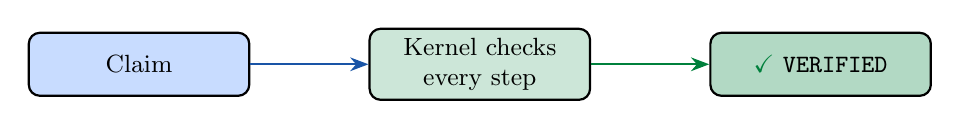
\begin{tikzpicture}[
  box/.style={draw, thick, rounded corners, minimum width=2.8cm,
              minimum height=0.8cm, font=\small, align=center}
]
  \node[box, fill=jugeoLight]                       (claim) {Claim};
  \node[box, fill=jugeoGreen!20, right=1.5cm of claim] (kern) {Kernel checks\\every step};
  \node[box, fill=jugeoGreen!30, right=1.5cm of kern]  (ok)   {\textcolor{jugeoGreen}{\checkmark}~\texttt{VERIFIED}};

  \draw[-{Stealth}, thick, jugeoBlue] (claim) -- (kern);
  \draw[-{Stealth}, thick, jugeoGreen] (kern) -- (ok);
\end{tikzpicture}
\end{center}
\vfill
\begin{itemize}
  \item No external dependency --- pure logical deduction
  \item Analogous to the verdict of a flawless DNA match
  \item \jugmark{Highest trust level in the system}
\end{itemize}
\end{frame}

% ---------------------------------------------------------------------------
% Slide 47: Trust Level — SOLVER_DISCHARGED
% ---------------------------------------------------------------------------
\begin{frame}
\frametitle{Trust Level --- \texttt{SOLVER\_DISCHARGED}}
\begin{block}{SMT Solver Proved It}
Z3 (or another SMT solver) automatically proved the claim.\\
\textbf{Very high confidence} --- but depends on Z3's own correctness.
\end{block}
\vspace{0.3cm}
\begin{center}
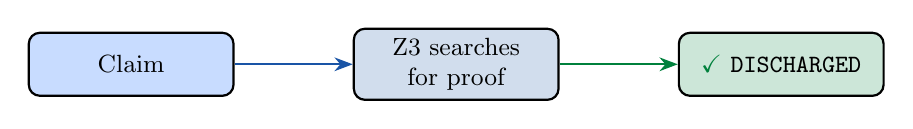
\begin{tikzpicture}[
  box/.style={draw, thick, rounded corners, minimum width=2.6cm,
              minimum height=0.8cm, font=\small, align=center}
]
  \node[box, fill=jugeoLight]                        (claim) {Claim};
  \node[box, fill=jugeoBlue!20, right=1.5cm of claim]  (z3)   {Z3 searches\\for proof};
  \node[box, fill=jugeoGreen!20, right=1.5cm of z3]    (ok)   {\textcolor{jugeoGreen}{\checkmark}~\texttt{DISCHARGED}};

  \draw[-{Stealth}, thick, jugeoBlue] (claim) -- (z3);
  \draw[-{Stealth}, thick, jugeoGreen] (z3) -- (ok);
\end{tikzpicture}
\end{center}
\vfill
\begin{itemize}
  \item Z3 is powerful but not infallible (solver bugs, bit-blasting limits)
  \item Excellent for arithmetic, array bounds, linear constraints
  \item \jugmark{One step below a full kernel proof}
\end{itemize}
\end{frame}

% ---------------------------------------------------------------------------
% Slide 48: Trust Level — RUNTIME_WITNESSED
% ---------------------------------------------------------------------------
\begin{frame}
\frametitle{Trust Level --- \texttt{RUNTIME\_WITNESSED}}
\begin{block}{Tests Ran and Passed}
Dynamic evidence: the claim held for \emph{all tested inputs}.\\
Good evidence, but \textbf{only covers the tested cases}.
\end{block}
\vspace{0.3cm}
\begin{center}
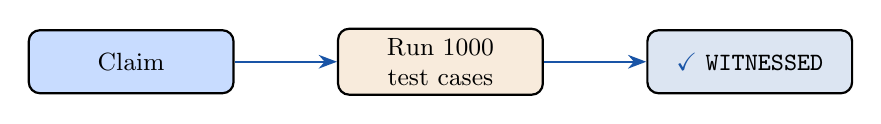
\begin{tikzpicture}[
  box/.style={draw, thick, rounded corners, minimum width=2.6cm,
              minimum height=0.8cm, font=\small, align=center}
]
  \node[box, fill=jugeoLight]                          (claim) {Claim};
  \node[box, fill=jugeoOrange!15, right=1.3cm of claim]  (run)  {Run 1000\\test cases};
  \node[box, fill=jugeoBlue!15, right=1.3cm of run]      (ok)   {\textcolor{jugeoBlue}{\checkmark}~\texttt{WITNESSED}};

  \draw[-{Stealth}, thick, jugeoBlue] (claim) -- (run);
  \draw[-{Stealth}, thick, jugeoBlue] (run) -- (ok);
\end{tikzpicture}
\end{center}
\vfill
\begin{itemize}
  \item ``I checked 1\,000 cases and they all worked''
  \item Does \textbf{not} guarantee the 1\,001st case
  \item Useful when solvers time out or formal proof is too expensive
  \item \jugmark{Honest about its limits --- unlike ``all tests pass = correct''}
\end{itemize}
\end{frame}

% ---------------------------------------------------------------------------
% Slide 49: Trust Level — COPILOT_SUGGESTED
% ---------------------------------------------------------------------------
\begin{frame}
\frametitle{Trust Level --- \texttt{COPILOT\_SUGGESTED}}
\begin{alertblock}{An AI Suggested This Is Correct}
A language model (e.g.\ GitHub Copilot) proposed the claim or invariant.\\
Useful hint, but \textbf{NOT} a proof.
\end{alertblock}
\vspace{0.3cm}
\begin{center}
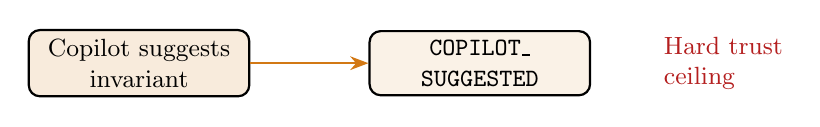
\begin{tikzpicture}[
  box/.style={draw, thick, rounded corners, minimum width=2.8cm,
              minimum height=0.8cm, font=\small, align=center}
]
  \node[box, fill=jugeoOrange!15]                        (ai) {Copilot suggests\\invariant};
  \node[box, fill=jugeoOrange!10, right=1.5cm of ai]     (tag) {\texttt{COPILOT\_}\\
                                                                  \texttt{SUGGESTED}};
  \node[right=0.8cm of tag, font=\small, text=jugeoRed, align=left]
    {Hard trust\\ceiling};

  \draw[-{Stealth}, thick, jugeoOrange] (ai) -- (tag);
\end{tikzpicture}
\end{center}
\vfill
\begin{itemize}
  \item AI contributions are \jugmark{tracked, not banned}
  \item Cannot be silently promoted to \texttt{VERIFIED\_PROOF}
  \item Must be independently confirmed to raise trust level
\end{itemize}
\end{frame}

% ---------------------------------------------------------------------------
% Slide 50: Trust Level — The Lower Levels
% ---------------------------------------------------------------------------
\begin{frame}
\frametitle{Trust Levels --- The Lower Tiers}
\begin{columns}[T]
\begin{column}{0.32\textwidth}
\begin{block}{\texttt{ORACLE\_PROPOSED}}
  \begin{itemize}
    \item A human expert asserted this
    \item Reviewed but not mechanically checked
    \item ``Trust me, I'm a domain expert''
  \end{itemize}
\end{block}
\end{column}
\begin{column}{0.32\textwidth}
\begin{block}{\texttt{UNVERIFIED}}
  \begin{itemize}
    \item No evidence yet
    \item Default state for any new claim
    \item ``We haven't looked at this''
  \end{itemize}
\end{block}
\end{column}
\begin{column}{0.32\textwidth}
\begin{alertblock}{\texttt{CONTRADICTED}}
  \begin{itemize}
    \item Evidence \textbf{against} the claim
    \item A test failed, a counterexample found
    \item \textcolor{jugeoRed}{Cannot be ignored}
  \end{itemize}
\end{alertblock}
\end{column}
\end{columns}
\vfill
\begin{center}
\small \texttt{CONTRADICTED} is special: it \textbf{poisons} any composition it enters.\\
\jugmark{You cannot hide a known failure.}
\end{center}
\end{frame}

% ---------------------------------------------------------------------------
% Slide 51: The Trust Algebra — Formal Definition
% ---------------------------------------------------------------------------
\begin{frame}
\frametitle{The Trust Algebra --- Formal Definition}
\begin{center}
\vspace{0.2cm}
{\Large $\mathcal{T} = (E_{\mathrm{adm}},\;\leq,\;\oplus,\;\ominus,\;\uparrow,\;\downarrow)$}
\end{center}
\vspace{0.4cm}
\begin{center}
\small\textit{Don't panic!  We'll explain each piece.}
\end{center}
\vspace{0.3cm}
\begin{center}
\begin{tabular}{@{} c l @{}}
  \toprule
  \textbf{Symbol} & \textbf{Meaning} \\
  \midrule
  $E_{\mathrm{adm}}$ & The seven admissible trust levels \\
  $\leq$              & Ordering: \texttt{CONTRADICTED} $<$ \ldots\ $<$ \texttt{VERIFIED\_PROOF} \\
  $\oplus$            & \jugmark{Compose} evidence (take the weaker) \\
  $\ominus$           & \jugmark{Challenge} evidence (may demote) \\
  $\uparrow$          & \jugmark{Promote} (explicit, audited, never silent) \\
  $\downarrow$        & \jugmark{Demote} (when evidence is weakened) \\
  \bottomrule
\end{tabular}
\end{center}
\vfill
\begin{center}
\small Six operators, three laws, one guarantee: \jugmark{honest accounting}.
\end{center}
\end{frame}

% ---------------------------------------------------------------------------
% Slide 52: Operator — Composition (⊕)
% ---------------------------------------------------------------------------
\begin{frame}
\frametitle{Operator --- Composition ($\oplus$)}
\begin{block}{Rule: Take the Weaker Level}
When combining evidence from two channels, the result is the \textbf{minimum}.
\end{block}
\vspace{0.3cm}
\begin{center}
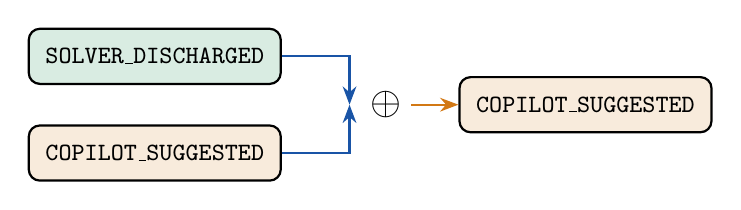
\begin{tikzpicture}[
  box/.style={draw, thick, rounded corners, minimum width=3.2cm,
              minimum height=0.7cm, font=\small, align=center}
]
  \node[box, fill=jugeoGreen!15]                       (a) {\texttt{SOLVER\_DISCHARGED}};
  \node[box, fill=jugeoOrange!15, below=0.5cm of a]   (b) {\texttt{COPILOT\_SUGGESTED}};
  \node[font=\Large, right=1cm of $(a.east)!0.5!(b.east)$] (op) {$\oplus$};
  \node[box, fill=jugeoOrange!15, right=0.6cm of op]  (r) {\texttt{COPILOT\_SUGGESTED}};

  \draw[-{Stealth}, thick, jugeoBlue] (a.east) -| ([xshift=-4pt]op.west);
  \draw[-{Stealth}, thick, jugeoBlue] (b.east) -| ([xshift=-4pt]op.west);
  \draw[-{Stealth}, thick, jugeoOrange] (op) -- (r);
\end{tikzpicture}
\end{center}
\vfill
\begin{center}
\Large\itshape ``A chain is only as strong as its weakest link.''
\end{center}
\end{frame}

% ---------------------------------------------------------------------------
% Slide 53: Why Weakest-Link?
% ---------------------------------------------------------------------------
\begin{frame}
\frametitle{Why Weakest-Link?}
\begin{exampleblock}{Scenario}
Z3 proved the \textbf{arithmetic} is correct.\\
A Copilot suggested the \textbf{loop invariant}.\\[4pt]
Your overall confidence is limited by the Copilot suggestion.
\end{exampleblock}
\vspace{0.4cm}
\begin{center}
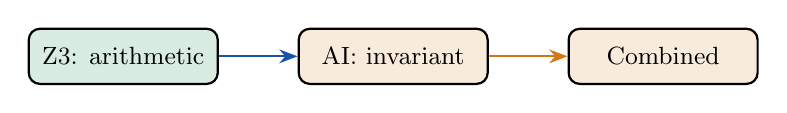
\begin{tikzpicture}[
  box/.style={draw, thick, rounded corners, minimum width=2.4cm,
              minimum height=0.7cm, font=\small, align=center}
]
  \node[box, fill=jugeoGreen!15]                        (z3)  {Z3: arithmetic};
  \node[box, fill=jugeoOrange!15, right=1cm of z3]      (cop) {AI: invariant};
  \node[box, fill=jugeoOrange!15, right=1cm of cop]     (all) {Combined};

  \draw[-{Stealth}, thick, jugeoBlue]   (z3)  -- (cop);
  \draw[-{Stealth}, thick, jugeoOrange] (cop) -- (all);
\end{tikzpicture}
\end{center}
\vfill
\begin{itemize}
  \item \textcolor{jugeoRed}{\textbf{You cannot launder low-trust evidence through high-trust channels}}
  \item The weakest link determines overall strength
  \item This is by design --- it keeps the system \jugmark{honest}
\end{itemize}
\end{frame}

% ---------------------------------------------------------------------------
% Slide 54: Law 1 — No Silent Promotion
% ---------------------------------------------------------------------------
\begin{frame}
\frametitle{Law 1 --- No Silent Promotion}
\begin{alertblock}{The Rule}
You \textbf{CANNOT} silently upgrade trust.  Every promotion requires:
\end{alertblock}
\vspace{0.3cm}
\begin{center}
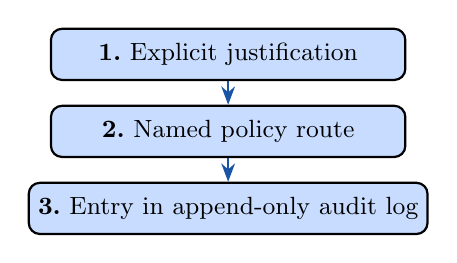
\begin{tikzpicture}[
  req/.style={draw, thick, rounded corners, fill=jugeoLight,
               minimum width=4.5cm, minimum height=0.65cm, font=\small}
]
  \node[req]                        (j) {\textbf{1.}~Explicit justification};
  \node[req, below=0.3cm of j]     (p) {\textbf{2.}~Named policy route};
  \node[req, below=0.3cm of p]     (a) {\textbf{3.}~Entry in append-only audit log};

  \draw[-{Stealth}, thick, jugeoBlue] (j) -- (p);
  \draw[-{Stealth}, thick, jugeoBlue] (p) -- (a);
\end{tikzpicture}
\end{center}
\vfill
\begin{itemize}
  \item Attempting silent promotion $\Rightarrow$ \textcolor{jugeoRed}{\texttt{JuGeoError}}
  \item The audit log is \textbf{append-only}: no rewriting history
  \item \jugmark{Trust must be earned, not assigned}
\end{itemize}
\end{frame}

% ---------------------------------------------------------------------------
% Slide 55: Code Example — Silent Promotion Fails
% ---------------------------------------------------------------------------
\begin{frame}[fragile]
\frametitle{Silent Promotion --- Fails}
\begin{lstlisting}[escapechar=@]
from jugeo.trust import TrustProfile, COPILOT_SUGGESTED, VERIFIED_PROOF

profile = TrustProfile(
    tier=COPILOT_SUGGESTED,
    source="copilot-invariant-suggestion",
    claim="loop_invariant_holds",
)

# Attempt silent promotion
profile.promote(VERIFIED_PROOF)
#  @\textcolor{jugeoRed}{\textrightarrow\ raises JuGeoError:}@
#  "Silent promotion from COPILOT_SUGGESTED
#   to VERIFIED_PROOF is forbidden.
#   Provide explicit=True with a reason."
\end{lstlisting}
\vfill
\begin{center}
\small The system \textbf{refuses} to upgrade trust without justification.\\
\jugmark{No shortcuts.}
\end{center}
\end{frame}

% ---------------------------------------------------------------------------
% Slide 56: Code Example — Explicit Promotion Works
% ---------------------------------------------------------------------------
\begin{frame}[fragile]
\frametitle{Explicit Promotion --- Works}
\begin{lstlisting}[escapechar=@]
from jugeo.trust import TrustProfile
from jugeo.trust import COPILOT_SUGGESTED, SOLVER_DISCHARGED

profile = TrustProfile(
    tier=COPILOT_SUGGESTED,
    source="copilot-invariant-suggestion",
)

# Explicit promotion with full justification
promoted = profile.promote(
    SOLVER_DISCHARGED,
    explicit=True,
    reason="z3-confirmed-arithmetic",
)
# @\textcolor{jugeoGreen}{\checkmark}@ promoted.tier == SOLVER_DISCHARGED
# @\textcolor{jugeoGreen}{\checkmark}@ Audit trail records promotion + reason
\end{lstlisting}
\vfill
\begin{center}
\small Every promotion is \jugmark{justified, named, and logged}.
\end{center}
\end{frame}

% ---------------------------------------------------------------------------
% Slide 57: Law 2 — Conservative Join
% ---------------------------------------------------------------------------
\begin{frame}
\frametitle{Law 2 --- Conservative Join}
\begin{block}{Rule: Always Take the Weaker Trust Level}
$a \oplus b = \min(a, b)$. This prevents \textbf{trust laundering}.
\end{block}
\vspace{0.2cm}
\begin{center}
\small
\begin{tabular}{@{} l c l c l @{}}
  \toprule
  \textbf{Channel A} & $\oplus$ & \textbf{Channel B} & $=$ & \textbf{Result} \\
  \midrule
  \texttt{VERIFIED\_PROOF}    & $\oplus$ & \texttt{VERIFIED\_PROOF}    & $=$ & \texttt{VERIFIED\_PROOF} \\
  \texttt{SOLVER\_DISCHARGED} & $\oplus$ & \texttt{RUNTIME\_WITNESSED} & $=$ & \texttt{RUNTIME\_WITNESSED} \\
  \texttt{SOLVER\_DISCHARGED} & $\oplus$ & \texttt{COPILOT\_SUGGESTED} & $=$ & \texttt{COPILOT\_SUGGESTED} \\
  \texttt{VERIFIED\_PROOF}    & $\oplus$ & \texttt{CONTRADICTED}       & $=$ & \texttt{CONTRADICTED} \\
  \bottomrule
\end{tabular}
\end{center}
\vfill
\begin{itemize}
  \item \texttt{CONTRADICTED} poisons everything --- you cannot ignore failure
  \item Composition is commutative: $a \oplus b = b \oplus a$
  \item \jugmark{No amount of strong evidence cancels a known contradiction}
\end{itemize}
\end{frame}

% ---------------------------------------------------------------------------
% Slide 58: Law 3 — Challenge Conservativity
% ---------------------------------------------------------------------------
\begin{frame}
\frametitle{Law 3 --- Challenge Conservativity}
\begin{alertblock}{Rule: Challenges May Demote, Never Ignore}
When evidence is challenged (e.g.\ a test fails), the system \textbf{must} respond.\\
Old trust cannot stand without explanation.
\end{alertblock}
\vspace{0.3cm}
\begin{center}
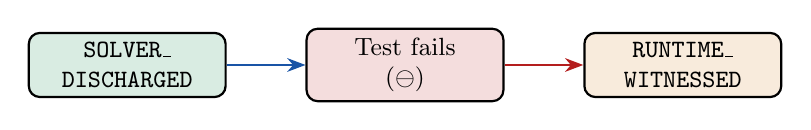
\begin{tikzpicture}[
  box/.style={draw, thick, rounded corners, minimum width=2.5cm,
              minimum height=0.7cm, font=\small, align=center}
]
  \node[box, fill=jugeoGreen!15]                         (before) {\texttt{SOLVER\_}\\
                                                                    \texttt{DISCHARGED}};
  \node[box, fill=jugeoRed!15, right=1cm of before]      (ch)     {Test fails\\($\ominus$)};
  \node[box, fill=jugeoOrange!15, right=1cm of ch]       (after)  {\texttt{RUNTIME\_}\\
                                                                    \texttt{WITNESSED}};

  \draw[-{Stealth}, thick, jugeoBlue] (before) -- (ch);
  \draw[-{Stealth}, thick, jugeoRed]  (ch) -- (after);
\end{tikzpicture}
\end{center}
\vfill
\begin{itemize}
  \item Like recalling a witness's testimony in court
  \item The demotion and its reason are logged in the audit trail
  \item \jugmark{The system never pretends a challenge didn't happen}
\end{itemize}
\end{frame}

% ---------------------------------------------------------------------------
% Slide 59: Why This Matters — A Real Scenario
% ---------------------------------------------------------------------------
\begin{frame}
\frametitle{A Real Scenario}
\begin{exampleblock}{Verifying \texttt{binary\_search}}
\small
\begin{description}[\textbf{Cover points:}]
  \item[\textbf{Cover points:}] 10 total obligations
  \item[\textbf{Z3 proved:}] 8 of 10 \hfill\textcolor{jugeoGreen}{\texttt{SOLVER\_DISCHARGED}}
  \item[\textbf{Z3 timed out:}] 2 edge cases \hfill\textcolor{jugeoOrange}{\texttt{---}}
  \item[\textbf{Runtime tests:}] confirmed the 2 edge cases \hfill\textcolor{jugeoBlue}{\texttt{RUNTIME\_WITNESSED}}
\end{description}
\end{exampleblock}
\vspace{0.3cm}
\begin{block}{JuGeo's Honest Report}
\begin{itemize}
  \item Overall trust: \texttt{RUNTIME\_WITNESSED} \hfill (conservative join)
  \item Residual obligations: \textbf{none}
  \item Every channel's contribution: \textbf{recorded}
\end{itemize}
\end{block}
\vfill
\begin{center}
\small Not ``fully proven'' --- but an \jugmark{honest, auditable account} of what was established and how.
\end{center}
\end{frame}

% ---------------------------------------------------------------------------
% Slide 60: Comparison — Trust Models
% ---------------------------------------------------------------------------
\begin{frame}
\frametitle{Trust Models --- Comparison}
\begin{center}
\begin{tabular}{@{} l c c c c @{}}
  \toprule
  & \textbf{LEAN} & \textbf{Coq} & \textbf{F*} & \jugmark{JuGeo} \\
  \midrule
  Trust levels       & 2 (binary)    & 2 (binary)    & 2 (binary)    & \textcolor{jugeoGreen}{\textbf{7}} \\
  Evidence channels  & 1             & 1             & 2 (SMT)       & \textcolor{jugeoGreen}{\textbf{6}} \\
  Audit trail        & \textcolor{jugeoRed}{No}  & \textcolor{jugeoRed}{No}  & \textcolor{jugeoRed}{No}  & \textcolor{jugeoGreen}{\textbf{Yes}} \\
  AI accounting      & \textcolor{jugeoRed}{No}  & \textcolor{jugeoRed}{No}  & \textcolor{jugeoRed}{No}  & \textcolor{jugeoGreen}{\textbf{Yes}} \\
  Challenge protocol & \textcolor{jugeoRed}{No}  & \textcolor{jugeoRed}{No}  & \textcolor{jugeoRed}{No}  & \textcolor{jugeoGreen}{\textbf{Yes}} \\
  Promotion control  & N/A           & N/A           & N/A           & \textcolor{jugeoGreen}{\textbf{Yes}} \\
  \bottomrule
\end{tabular}
\end{center}
\vfill
\begin{center}
\large JuGeo is the only system that gives you an\\
\jugmark{honest, multi-channel account of verification evidence}.
\end{center}
\end{frame}

\end{document}
%
